\documentclass{beamer}

\usepackage{graphicx}
\usepackage[galician]{babel}

\title{Experimentos e probas}
\author{TFG Pepe}
\setbeamertemplate{footline}[frame number]
\AtBeginSection[]
{
  \begin{frame}
    \frametitle{Indice}
    \tableofcontents[currentsection]
  \end{frame}
}

\AtBeginSubsection[]
{
  \begin{frame}
    \frametitle{Indice}
    \tableofcontents[currentsection,currentsubsection]
  \end{frame}
}


\definecolor{udcpink}{RGB}{177,0,114}
\setbeamercolor{structure}{fg=udcpink}


\begin{document}

\begin{frame}
  \titlepage
\end{frame}

\section{imagenet}
\begin{frame}

\frametitle{Proba de arquitecturas sobre Imagenet}

O experimento máis caro e custoso. Os artefactos xerados foron tamén examinados.

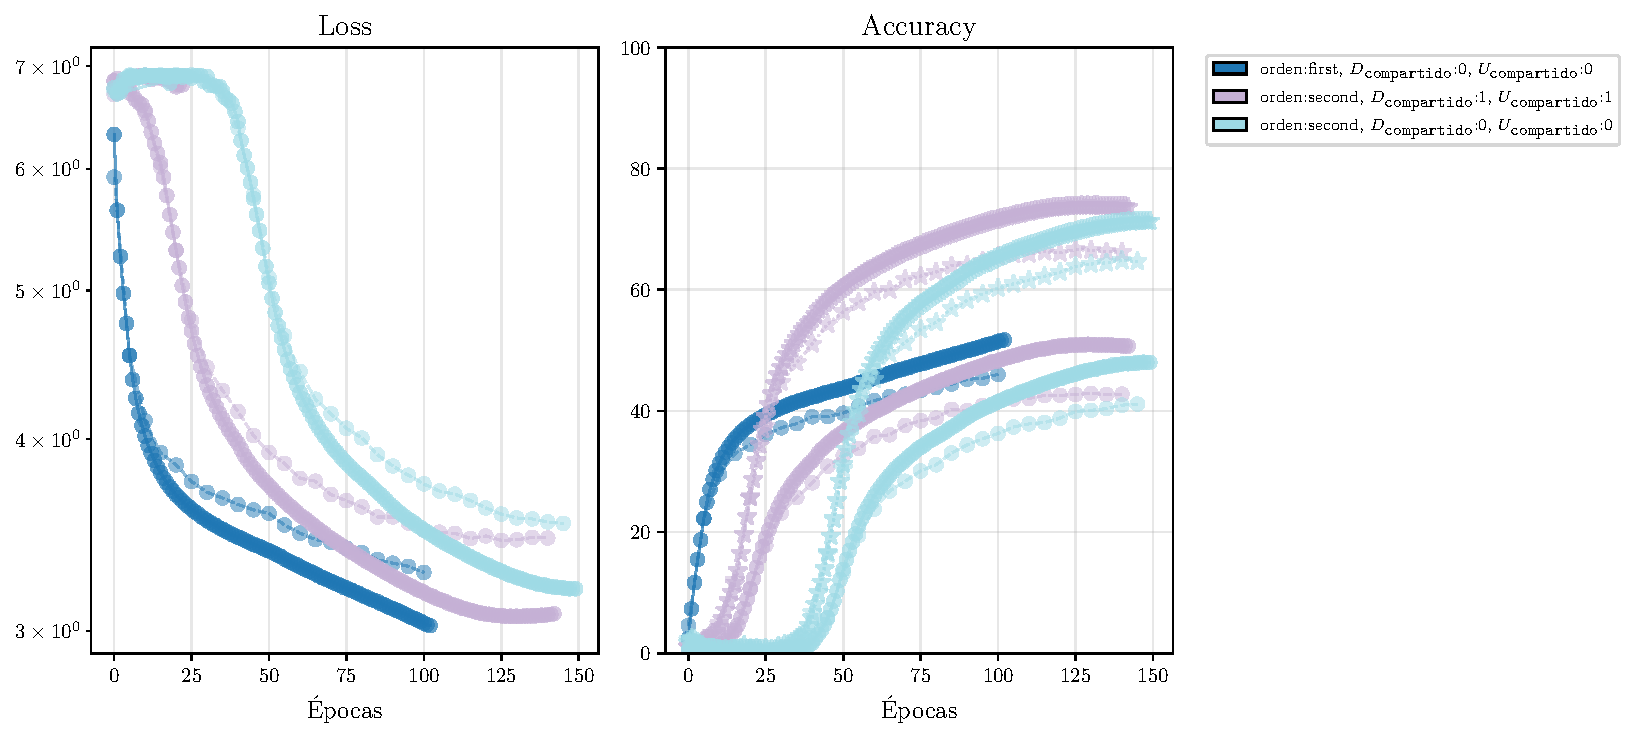
\includegraphics[width=0.9\textwidth]{imaxes/04471e_20ad3c_cd2702.pdf}

O certo é que os resultados parécenme \textbf{non} conlclusivos.
\end{frame}


\begin{frame}
\frametitle{Proba de arquitecturas sobre Imagenet - mcr2 e dispersión}

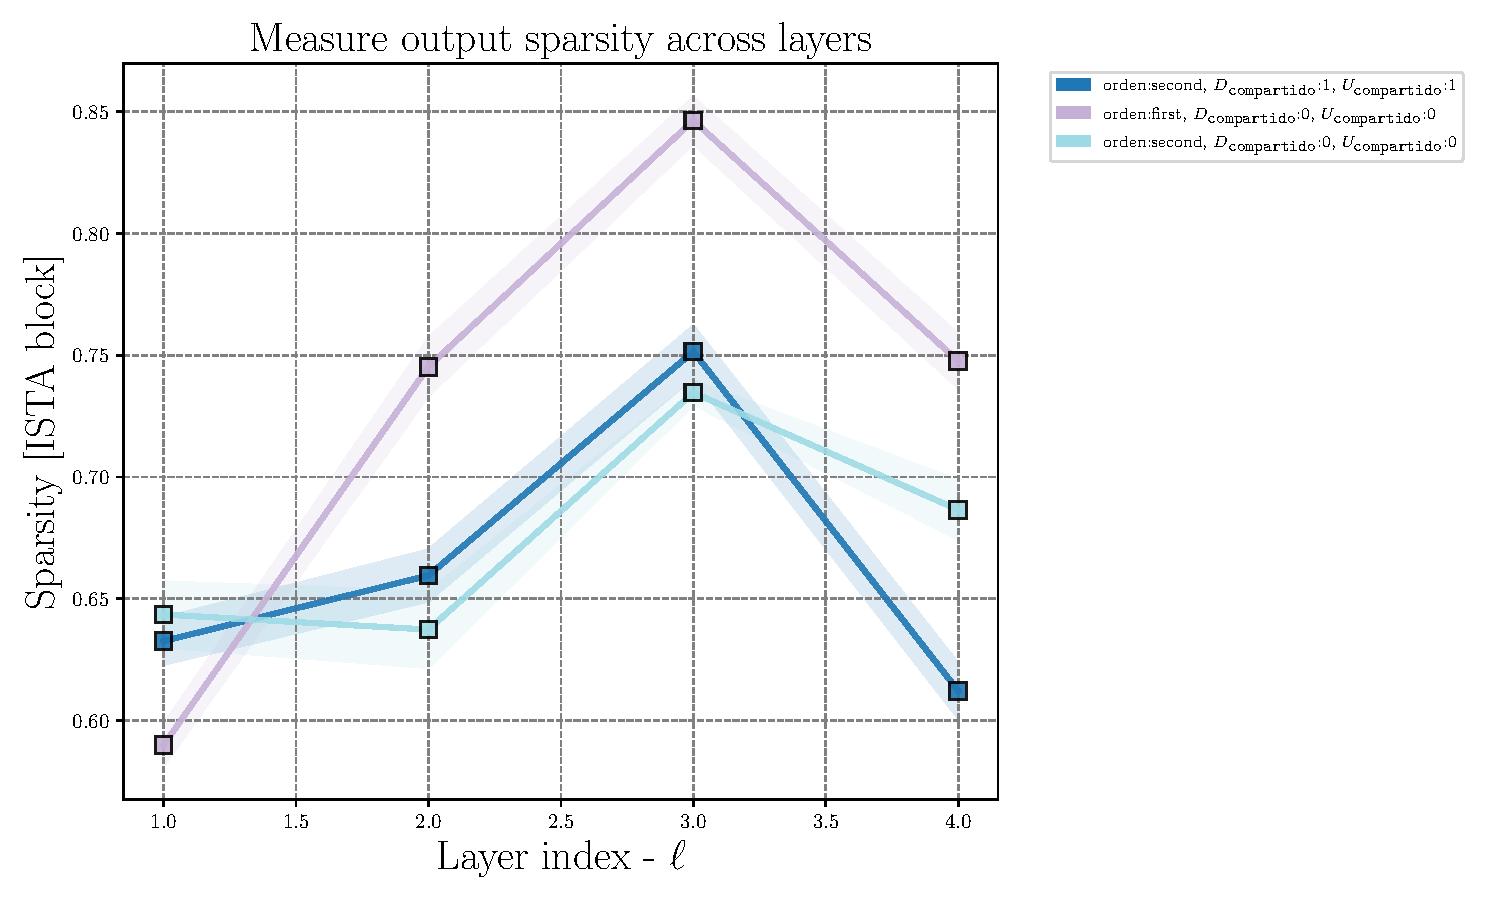
\includegraphics[width=0.48\textwidth]{imaxes/3b2194_01ee29_20ad3c_sparsity.pdf}\hfill
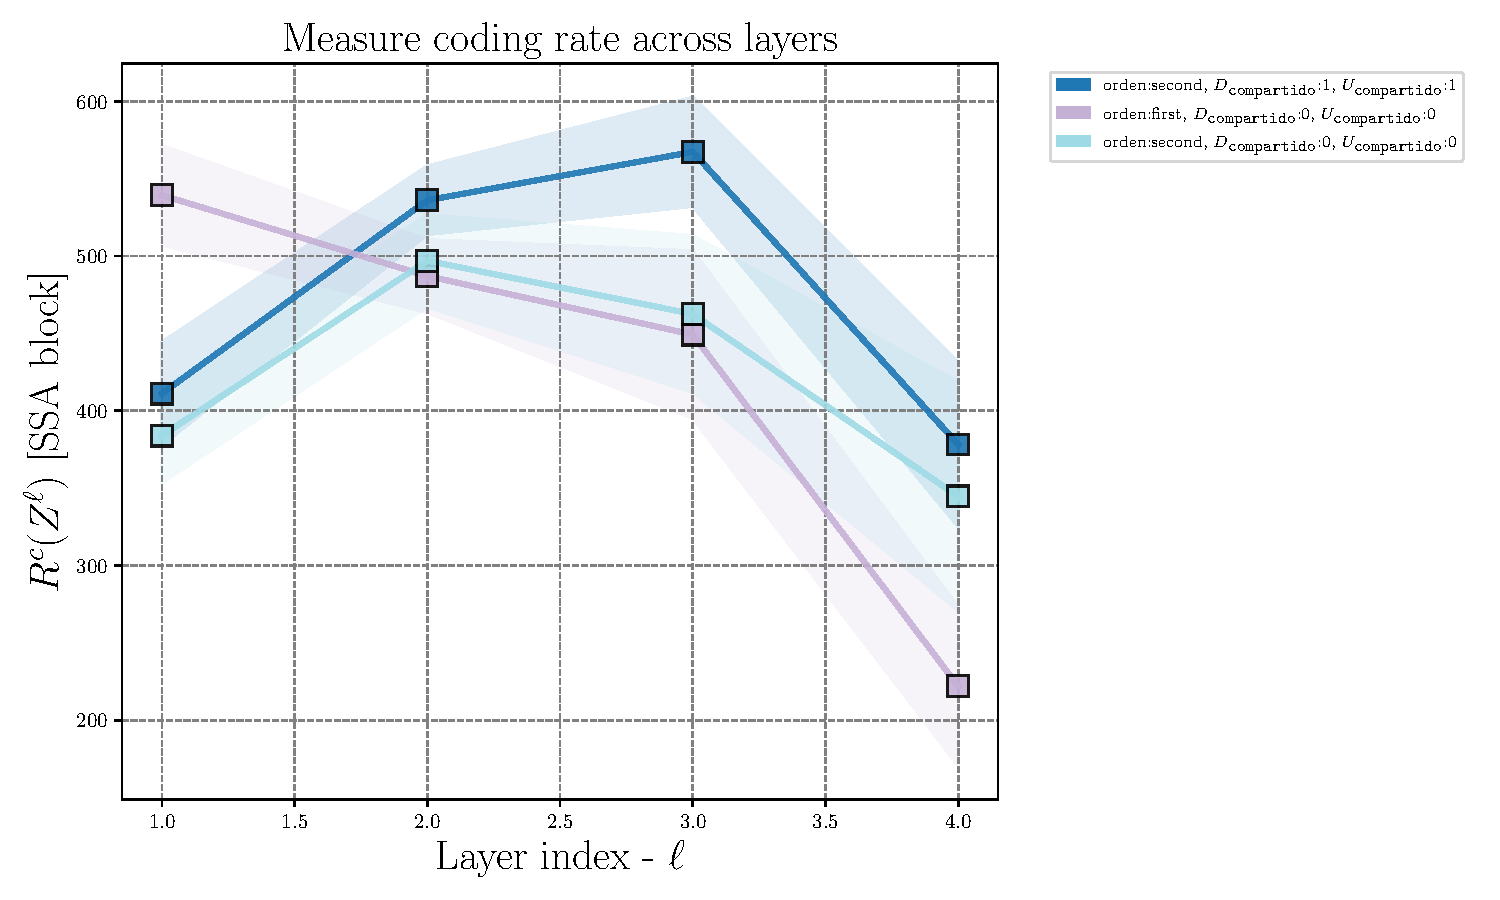
\includegraphics[width=0.48\textwidth]{imaxes/3b2194_01ee29_20ad3c_mcr2.pdf}

En ambas métricas a Rede orixinal é a millor. Non sabemos como sería a cousa con adestramentos máis longos. Entre as de segundo orden é un pouco millor a que non comparte.
\end{frame}

\begin{frame}
\frametitle{Proba de arquitecturas sobre Imagenet - parches representativos}
(izq) Segundo orden compartindo  (proposta) | (der)  Primeiro orden sen compartir (Yi Ma)

\includegraphics[width=0.48\textwidth]{imaxes/ret_img/01ee29.pth_retrieval.pdf}\hfill
\includegraphics[width=0.48\textwidth]{imaxes/ret_img/20ad3c.pth_retrieval.pdf}

De aquí non saco ningunha conclusión.

\end{frame}

\begin{frame}

\frametitle{Proba de arquitecturas sobre Imagenet - visualización da atención}

Primeiro e segundo orden respectivamente. Imaxes que o equipo de Yi Ma usa de demo.

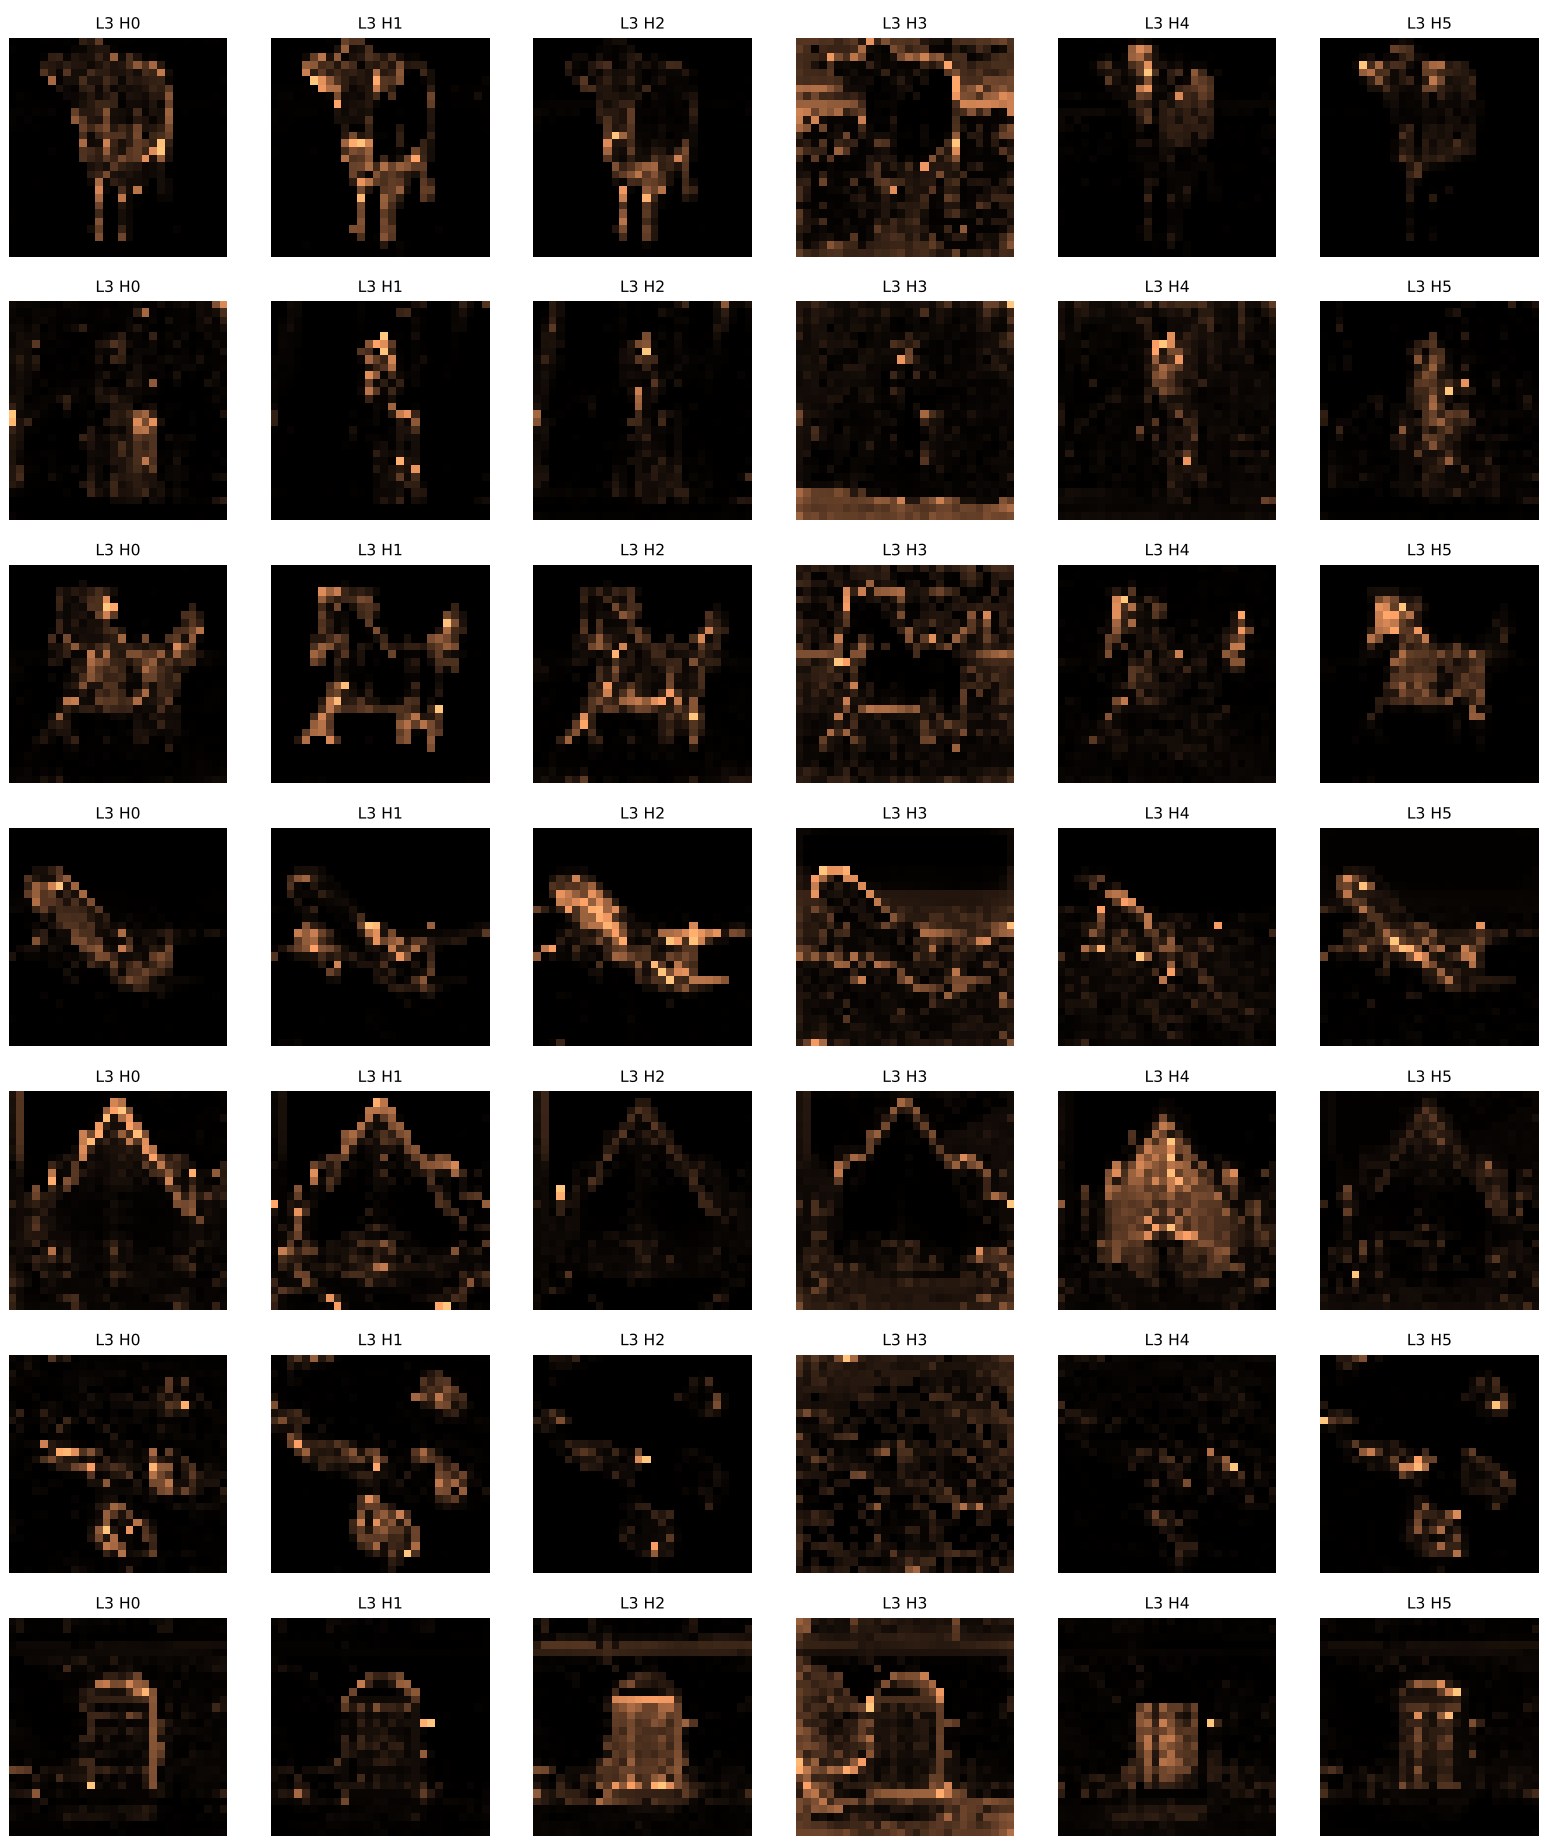
\includegraphics[width=0.37\textwidth]{imaxes/at_img/primerorden.png}\hfill
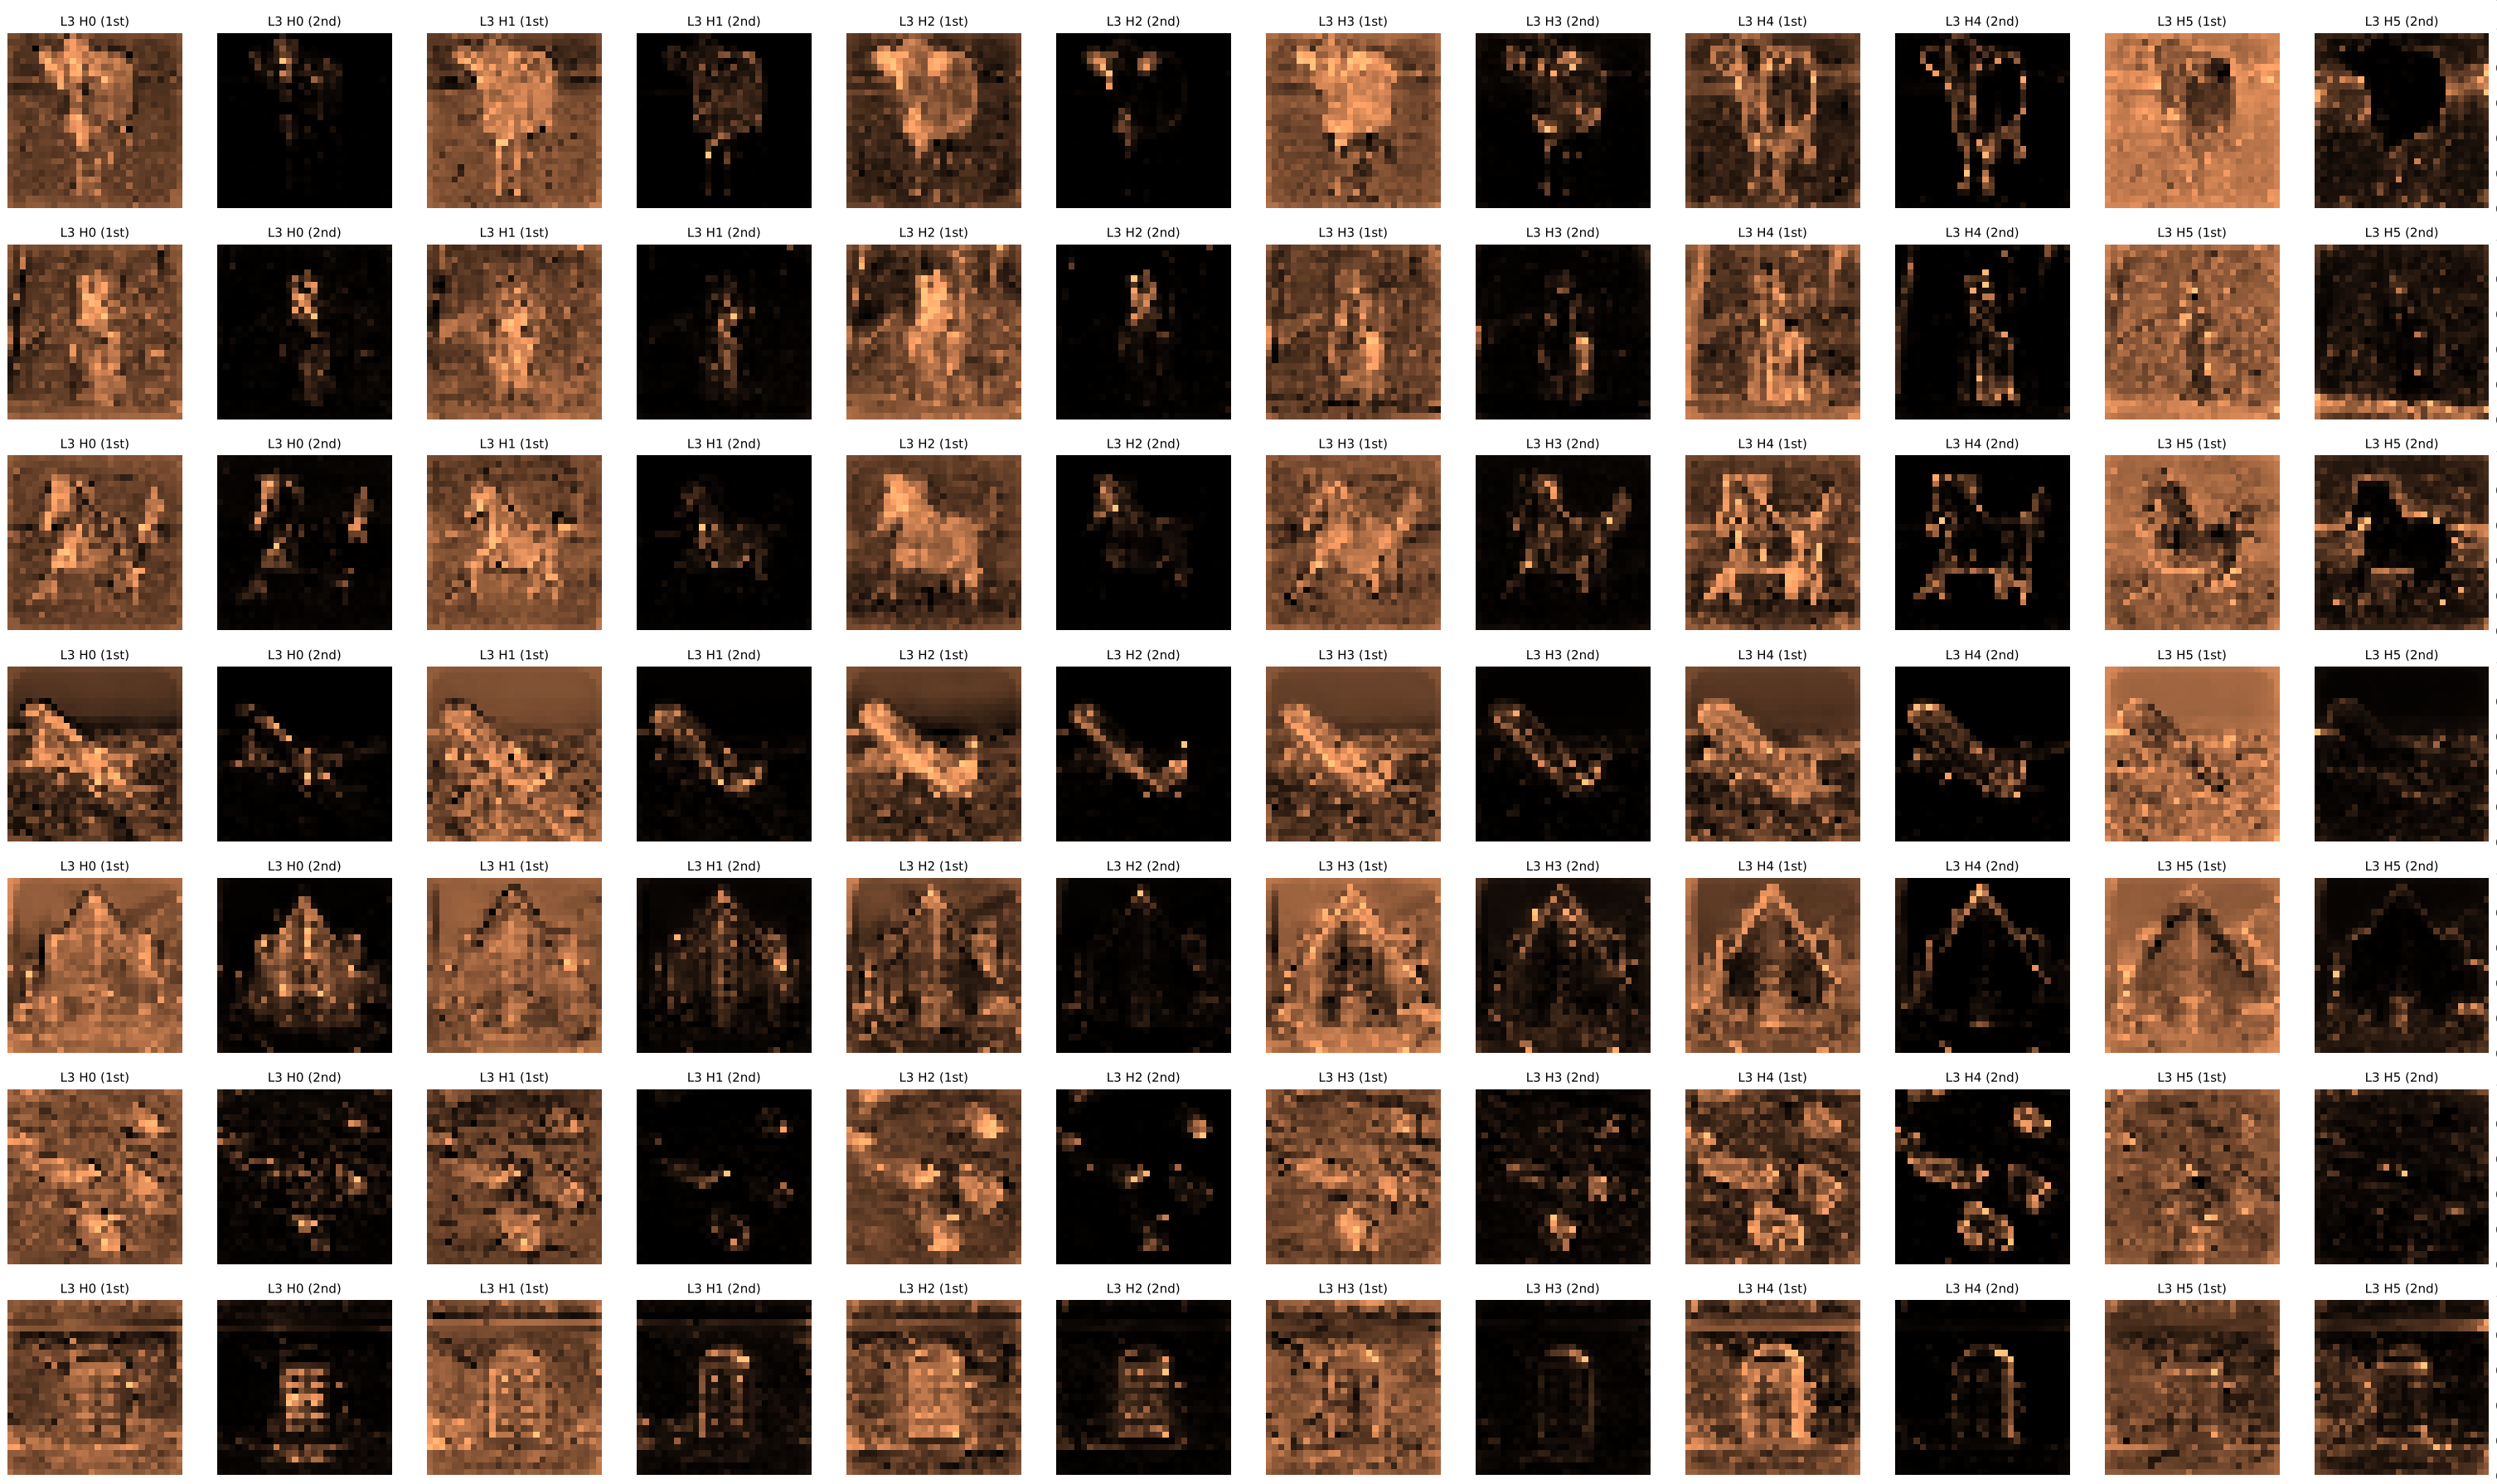
\includegraphics[width=0.60\textwidth]{imaxes/at_img/2ndorden.png}

\end{frame}

\begin{frame}

\frametitle{Proba de arquitecturas sobre Imagenet - visualización da atención}

Primeiro e segundo orden respectivamente. Imaxes de avellas e velutinas.

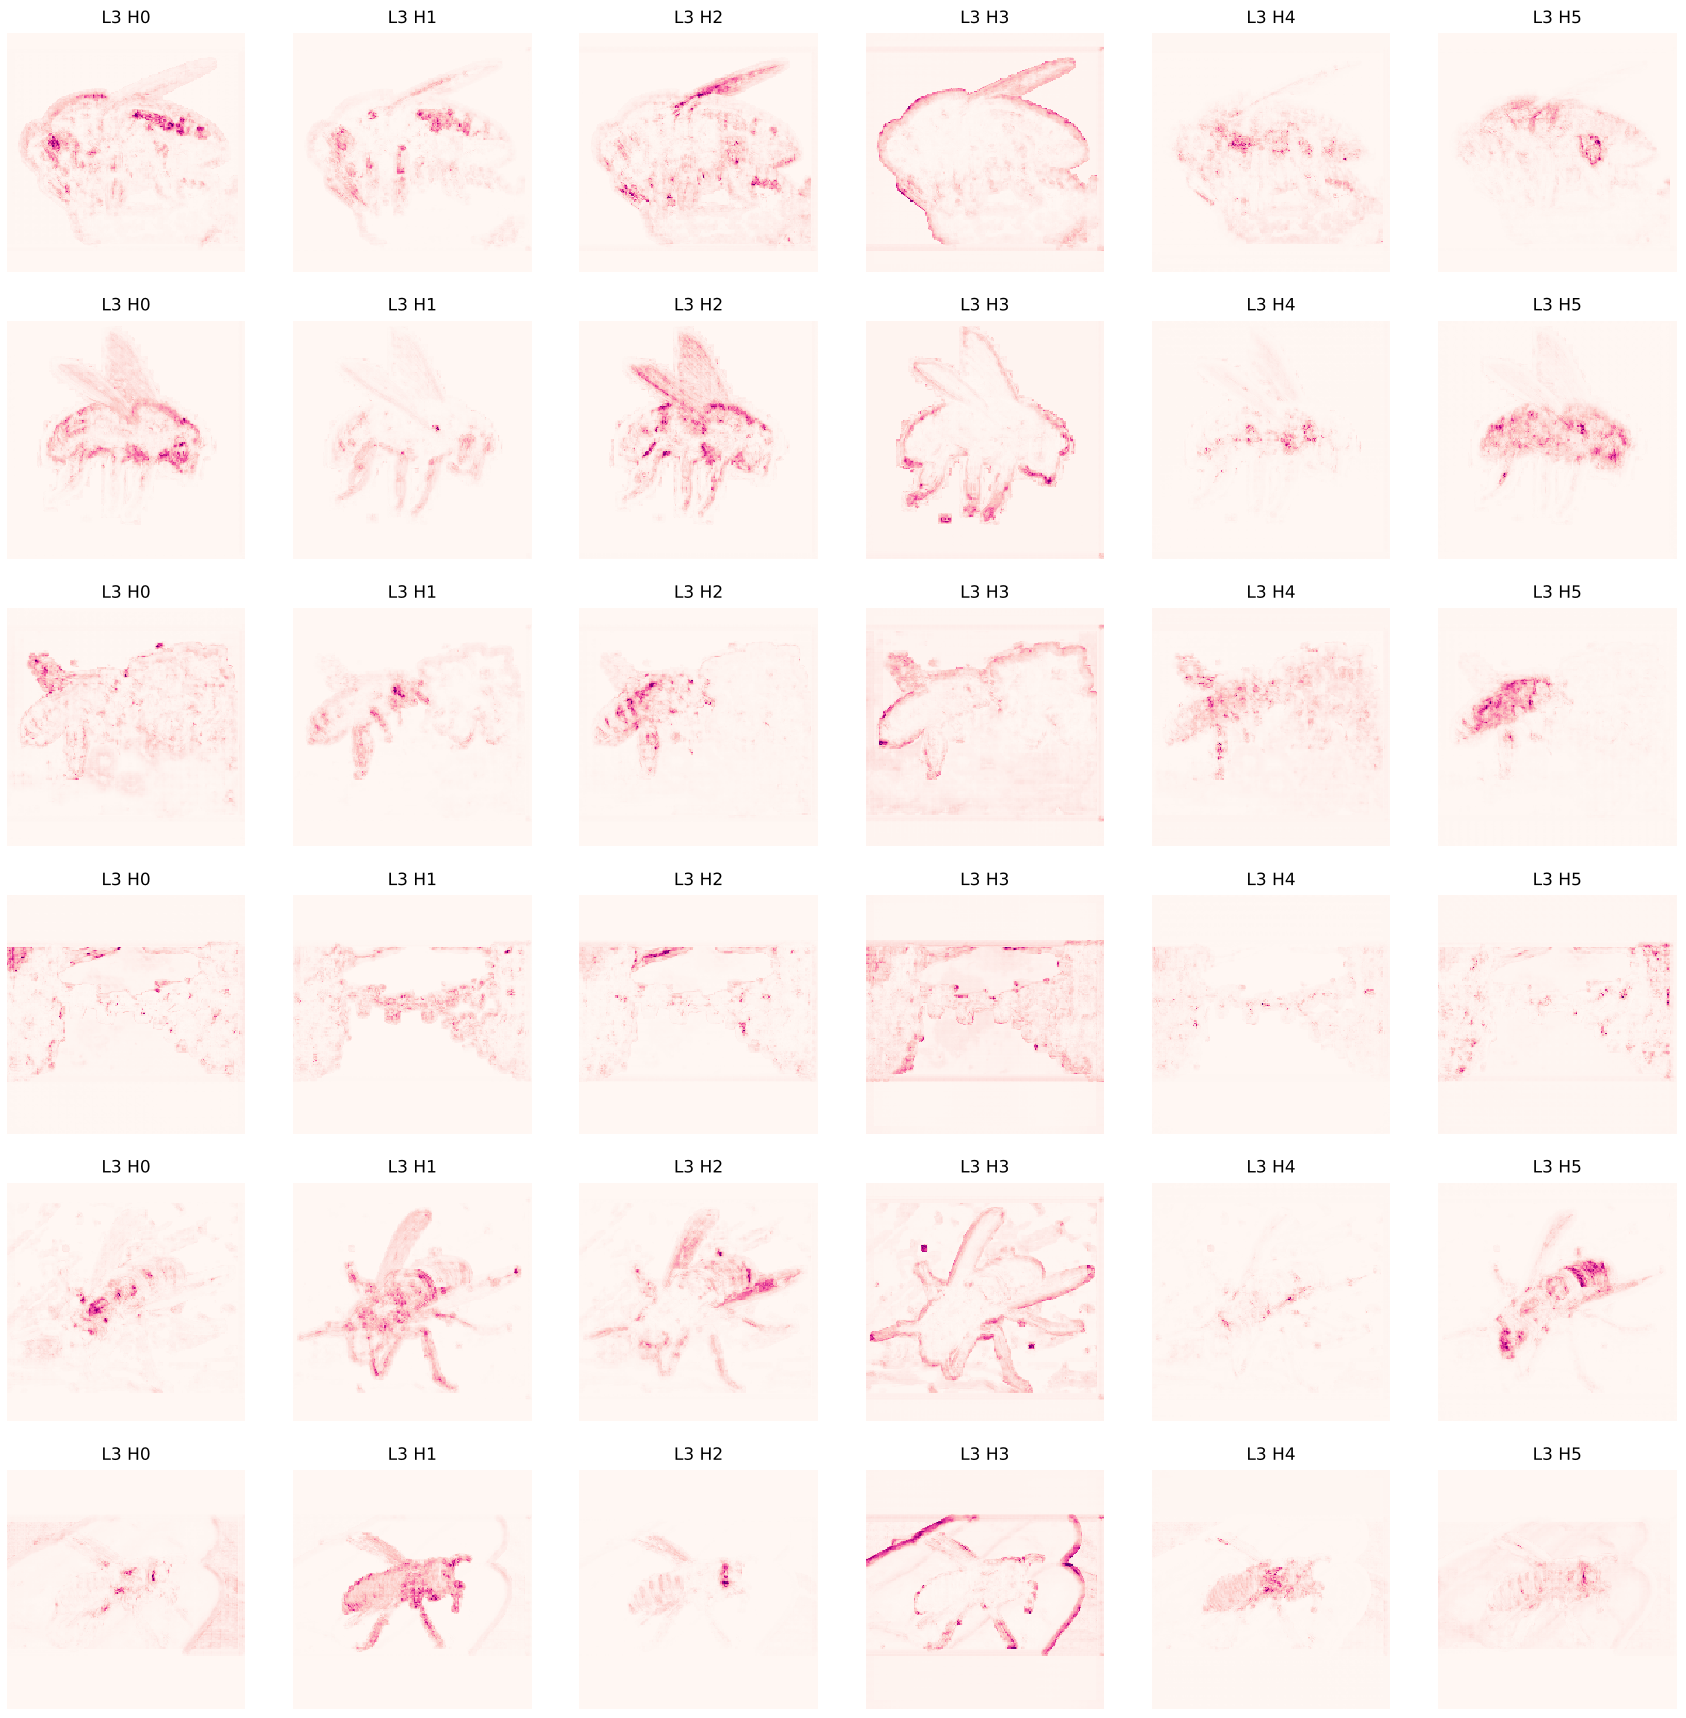
\includegraphics[width=0.37\textwidth]{imaxes/at_img/avellas1ro.png}\hfill
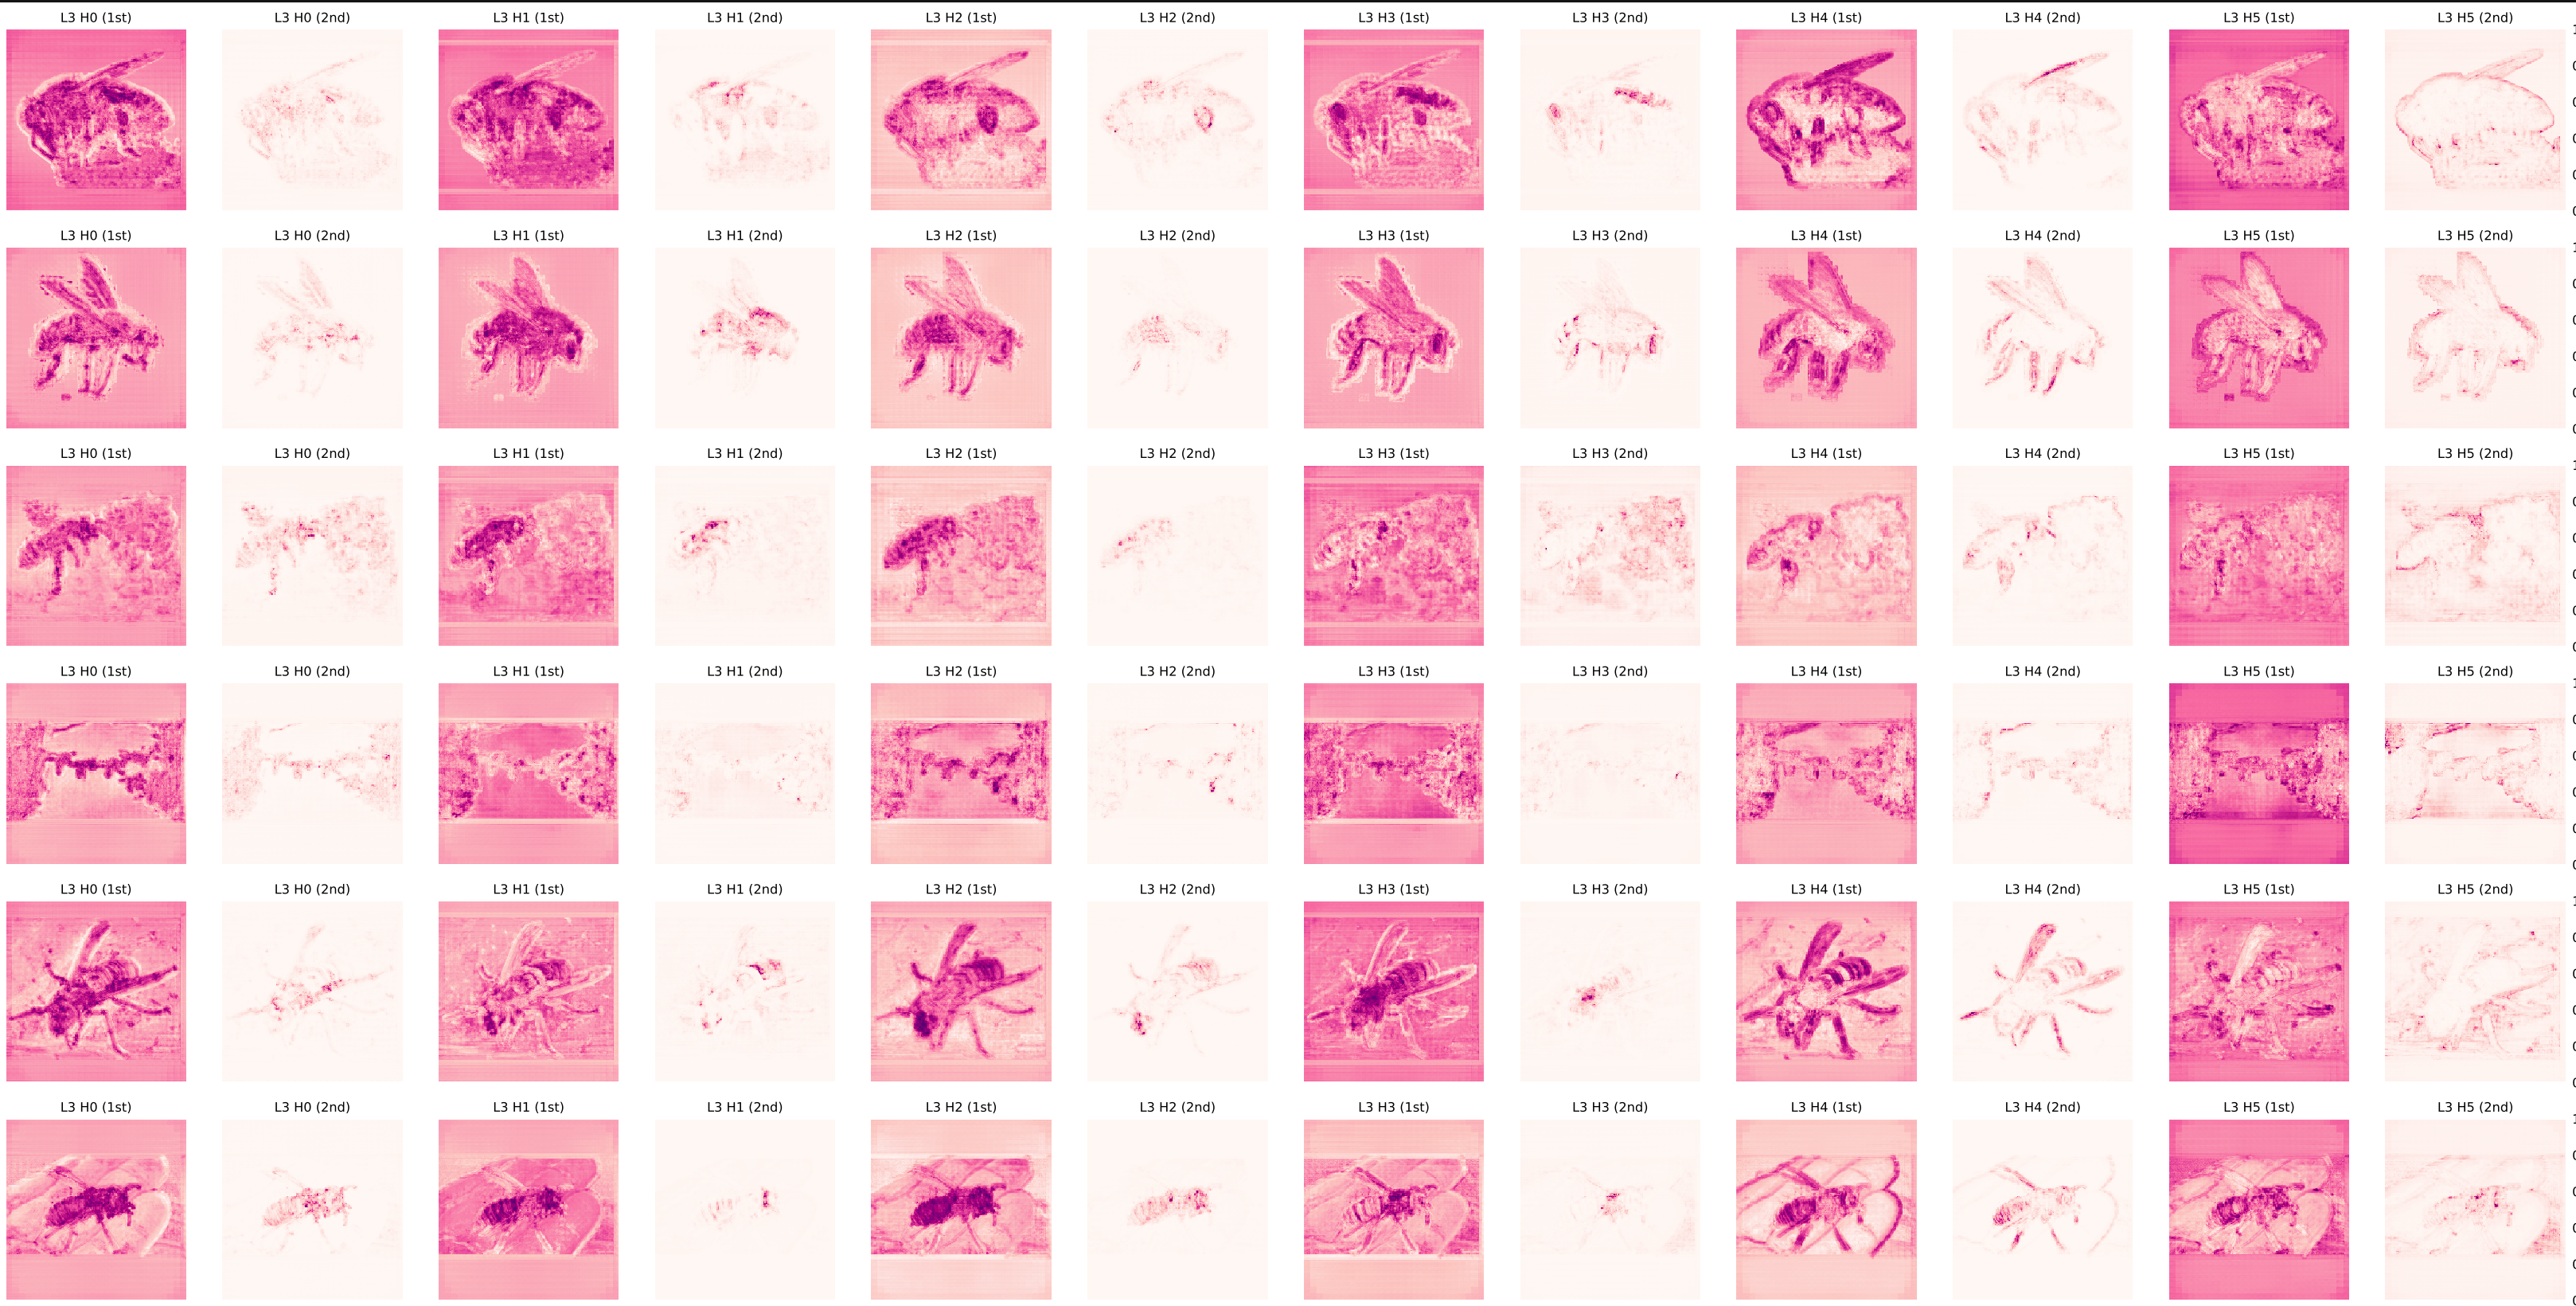
\includegraphics[width=0.60\textwidth]{imaxes/at_img/avellas2nd.png}

\end{frame}

\begin{frame}

\frametitle{Proba de arquitecturas sobre Imagenet - visualización da atención}

Primeiro e segundo orden respectivamente. Imaxes de vacas.

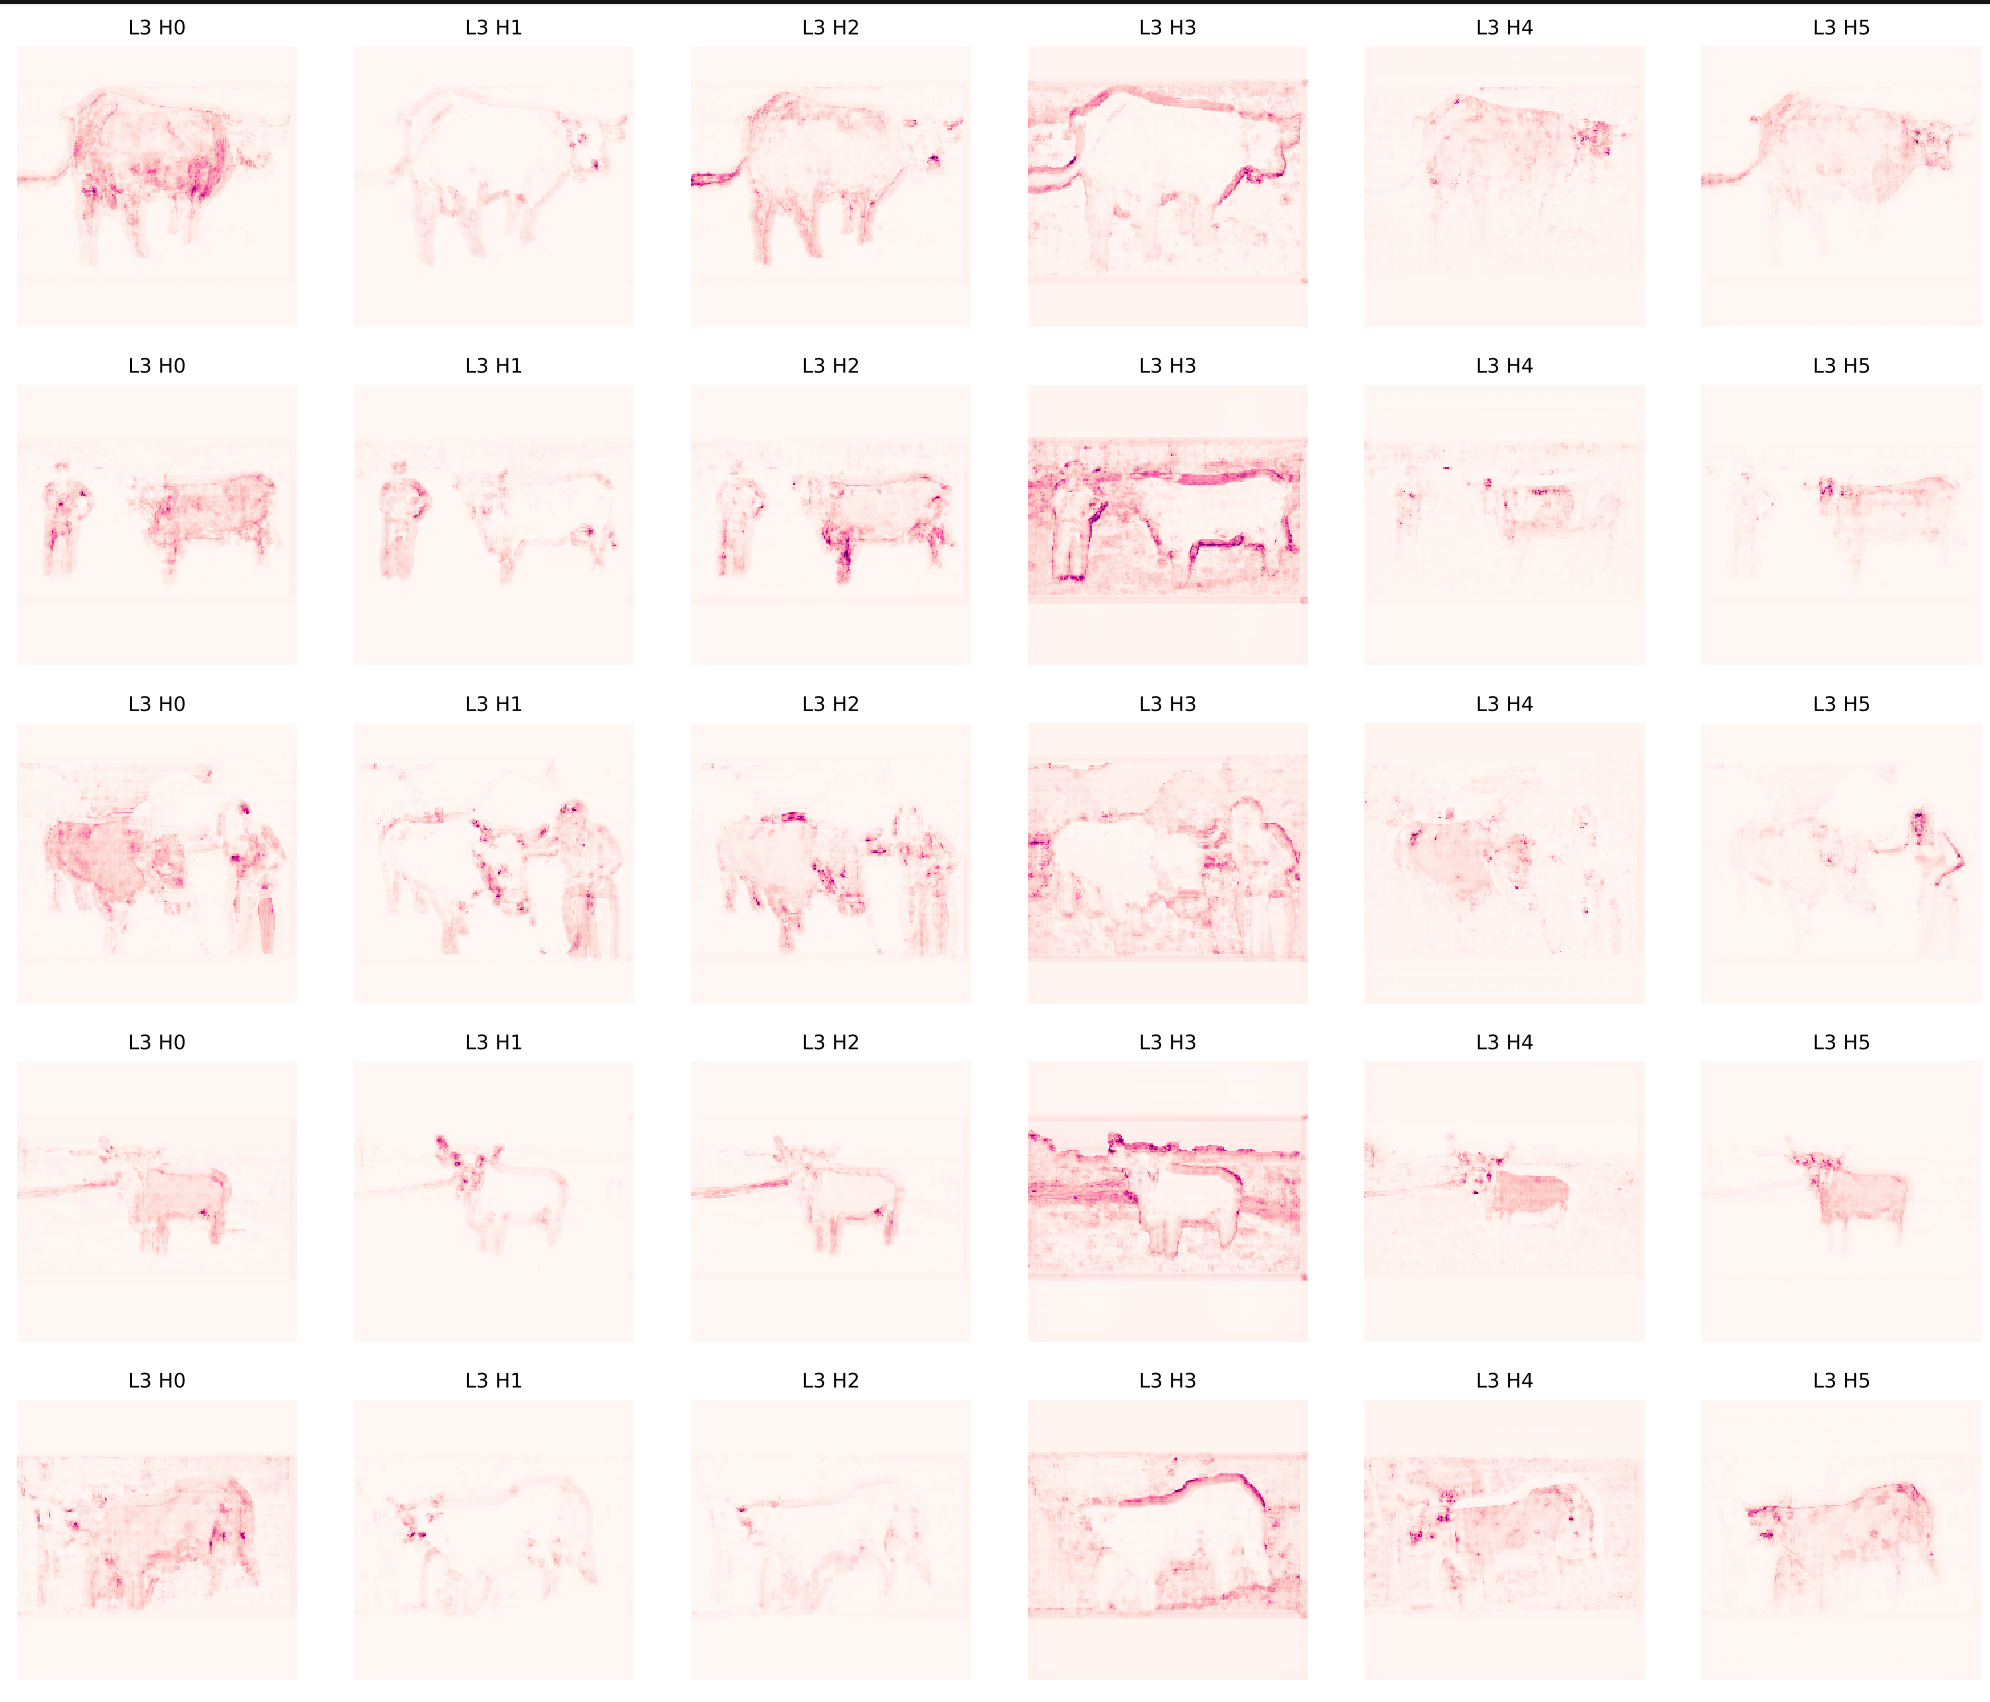
\includegraphics[width=0.37\textwidth]{imaxes/at_img/vacas1st.png}\hfill
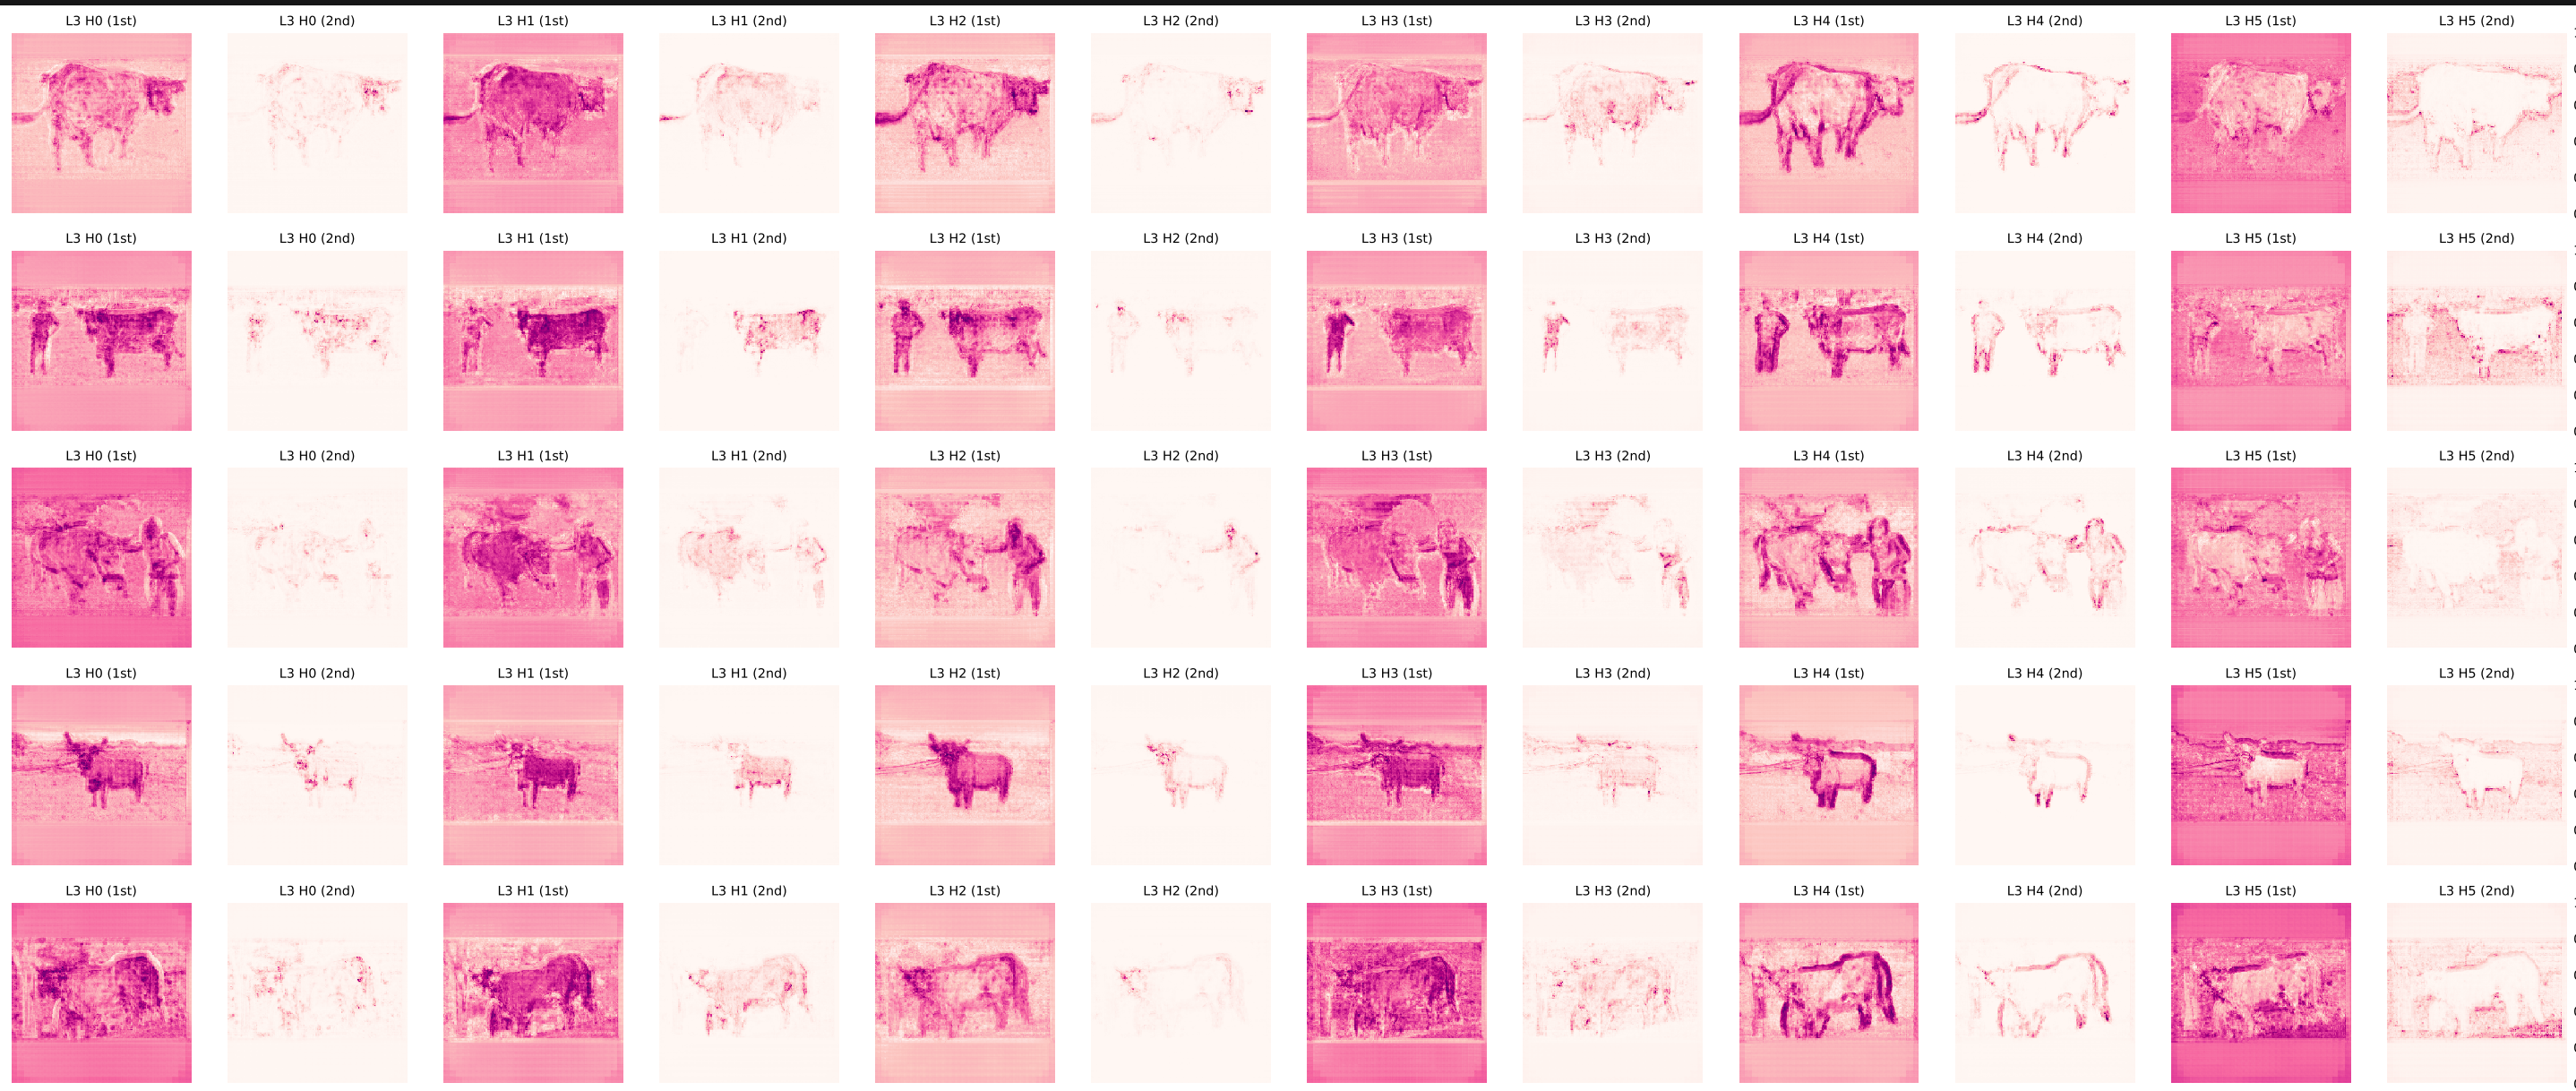
\includegraphics[width=0.60\textwidth]{imaxes/at_img/vacas2nd.png}

\end{frame}

\begin{frame}
\frametitle{Proba de arquitecturas sobre Imagenet - cruce de ordes}
(izq) primeiro inferencia segundo (der) segundo inferencia primeiro
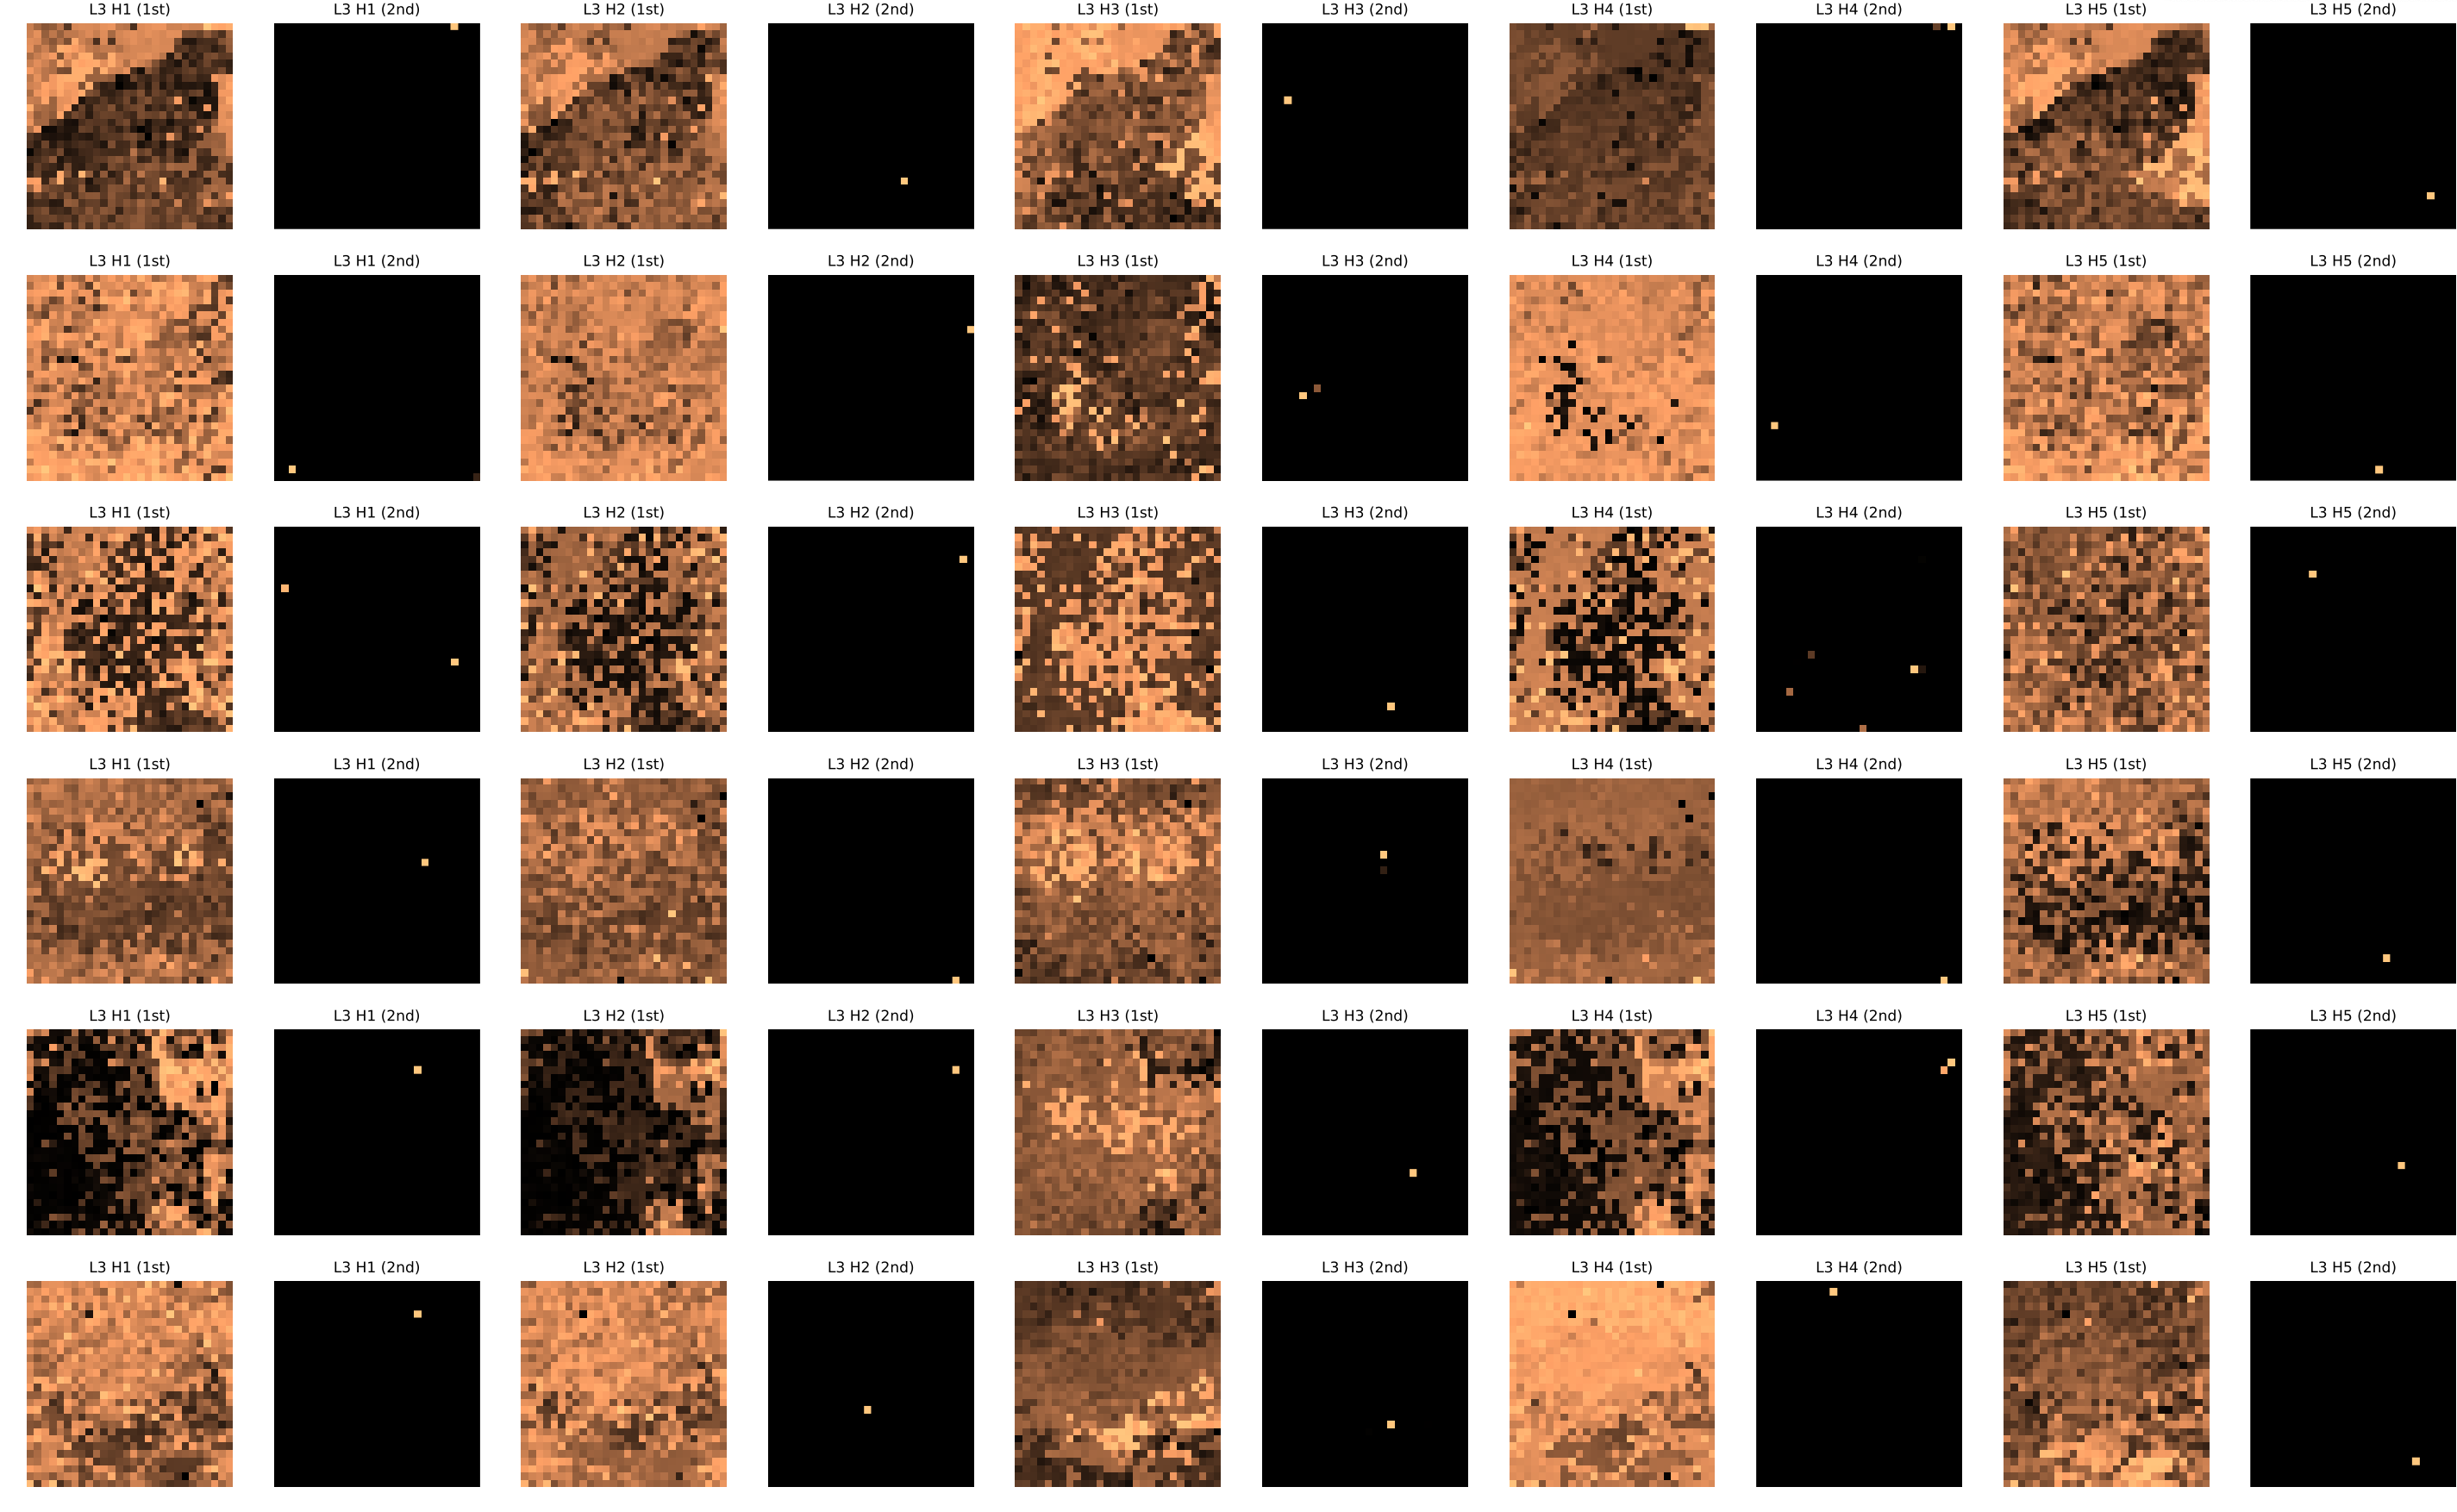
\includegraphics[width=0.60\textwidth]{imaxes/cruce_ord/1inf2.png}\hfill
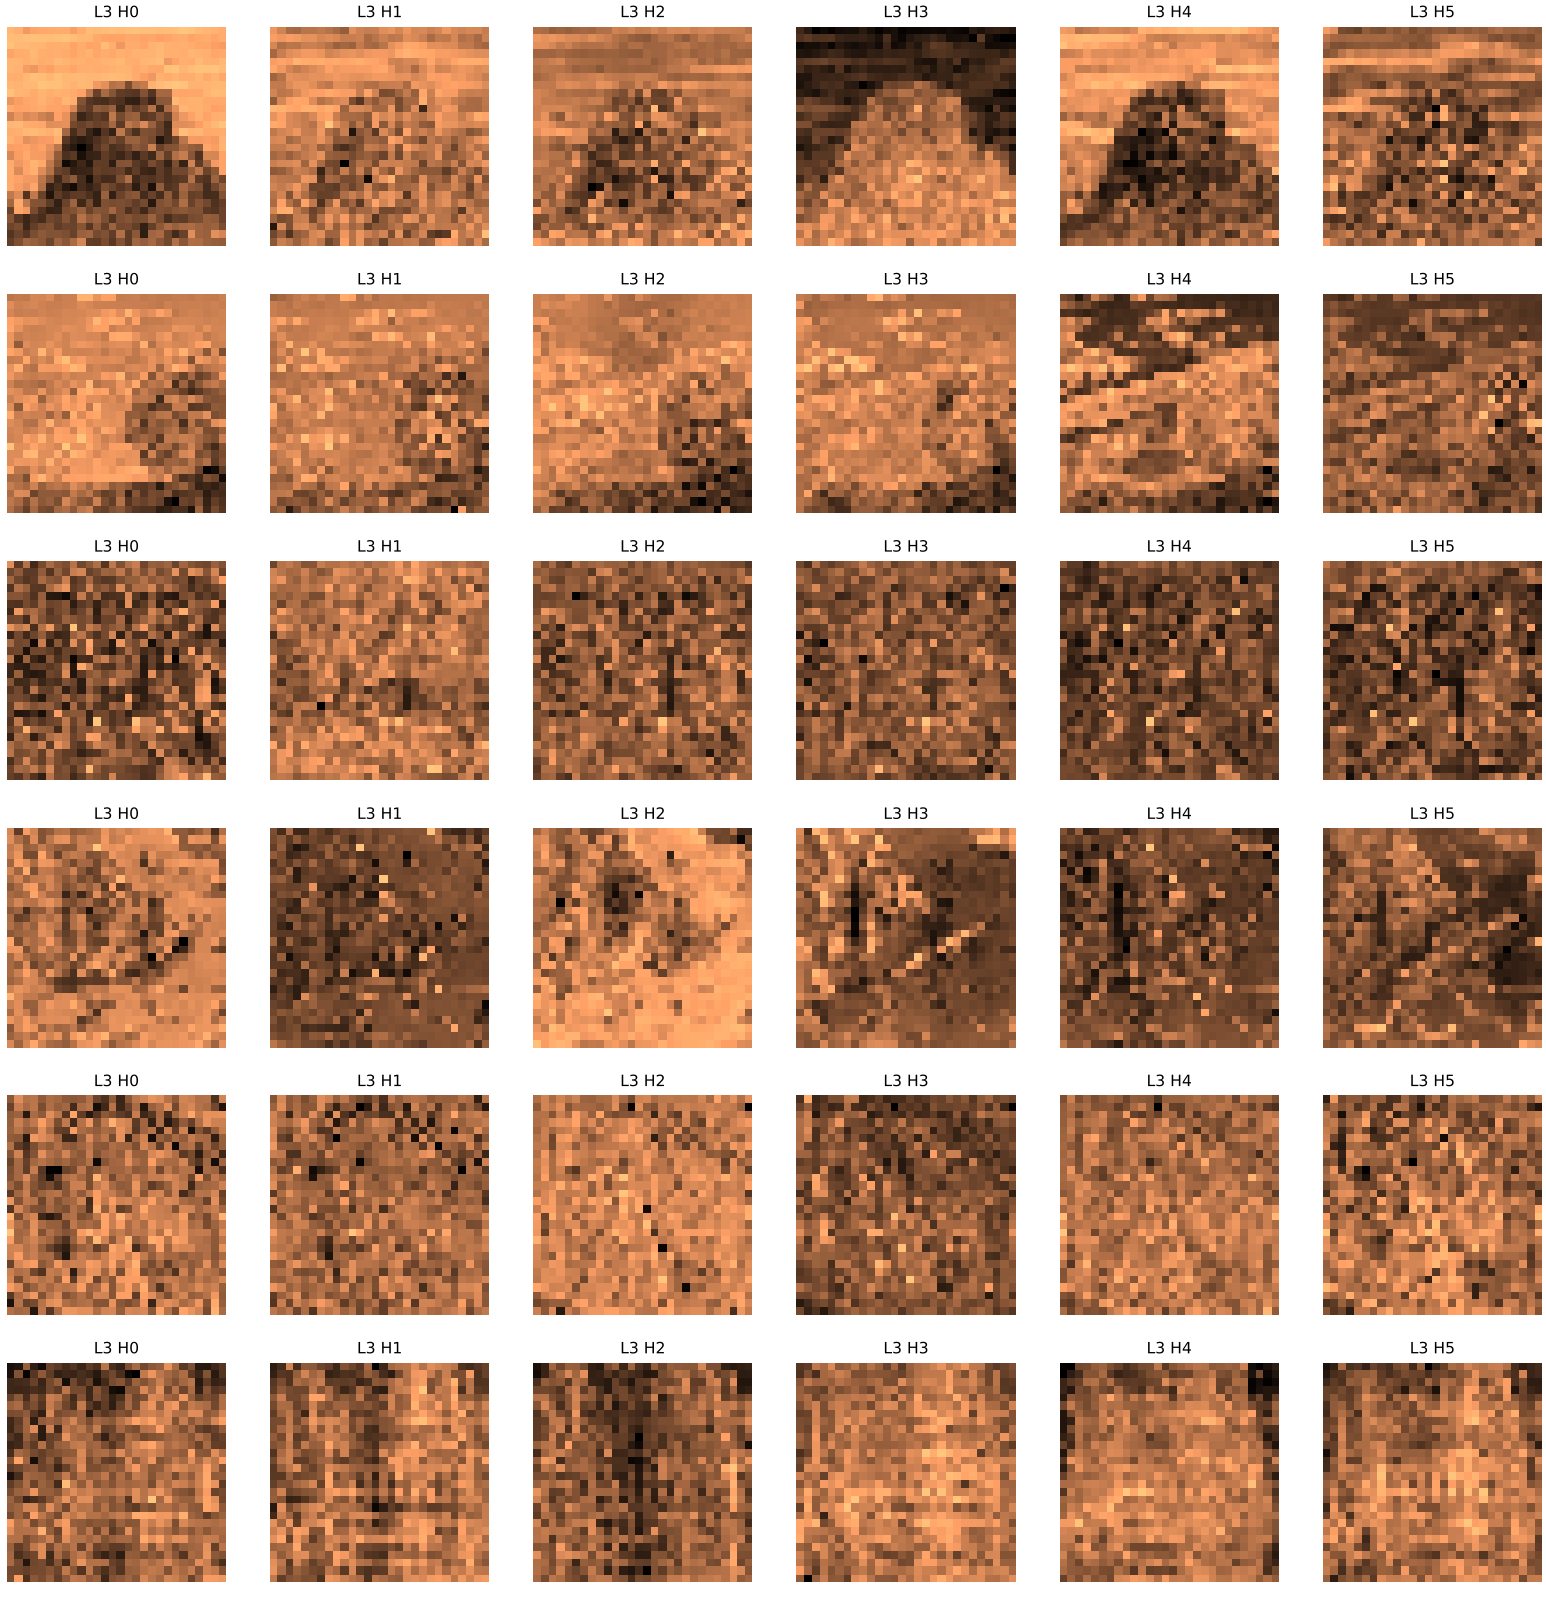
\includegraphics[width=0.35\textwidth]{imaxes/cruce_ord/2inf1.png}

\begin{table}[]
\begin{tabular}{|l|ll|ll|}
\hline
adestrado / inferencia & \multicolumn{2}{l|}{primeiro orden}  & \multicolumn{2}{l|}{segundo orden}   \\ \hline
                       & \multicolumn{1}{l|}{acc@1}  & acc@5  & \multicolumn{1}{l|}{acc@1}  & acc@5  \\ \hline
primeiro orden         & \multicolumn{1}{l|}{0.5260} & 0.7645 & \multicolumn{1}{l|}{0.0010} & 0.0052 \\ \hline
segundo orden          & \multicolumn{1}{l|}{0.0010} & 0.0055 & \multicolumn{1}{l|}{0.4721} & 0.7160 \\ \hline
\end{tabular}
\end{table}

\end{frame}


\section{drive}

\begin{frame}

\frametitle{a tarefa en sí}

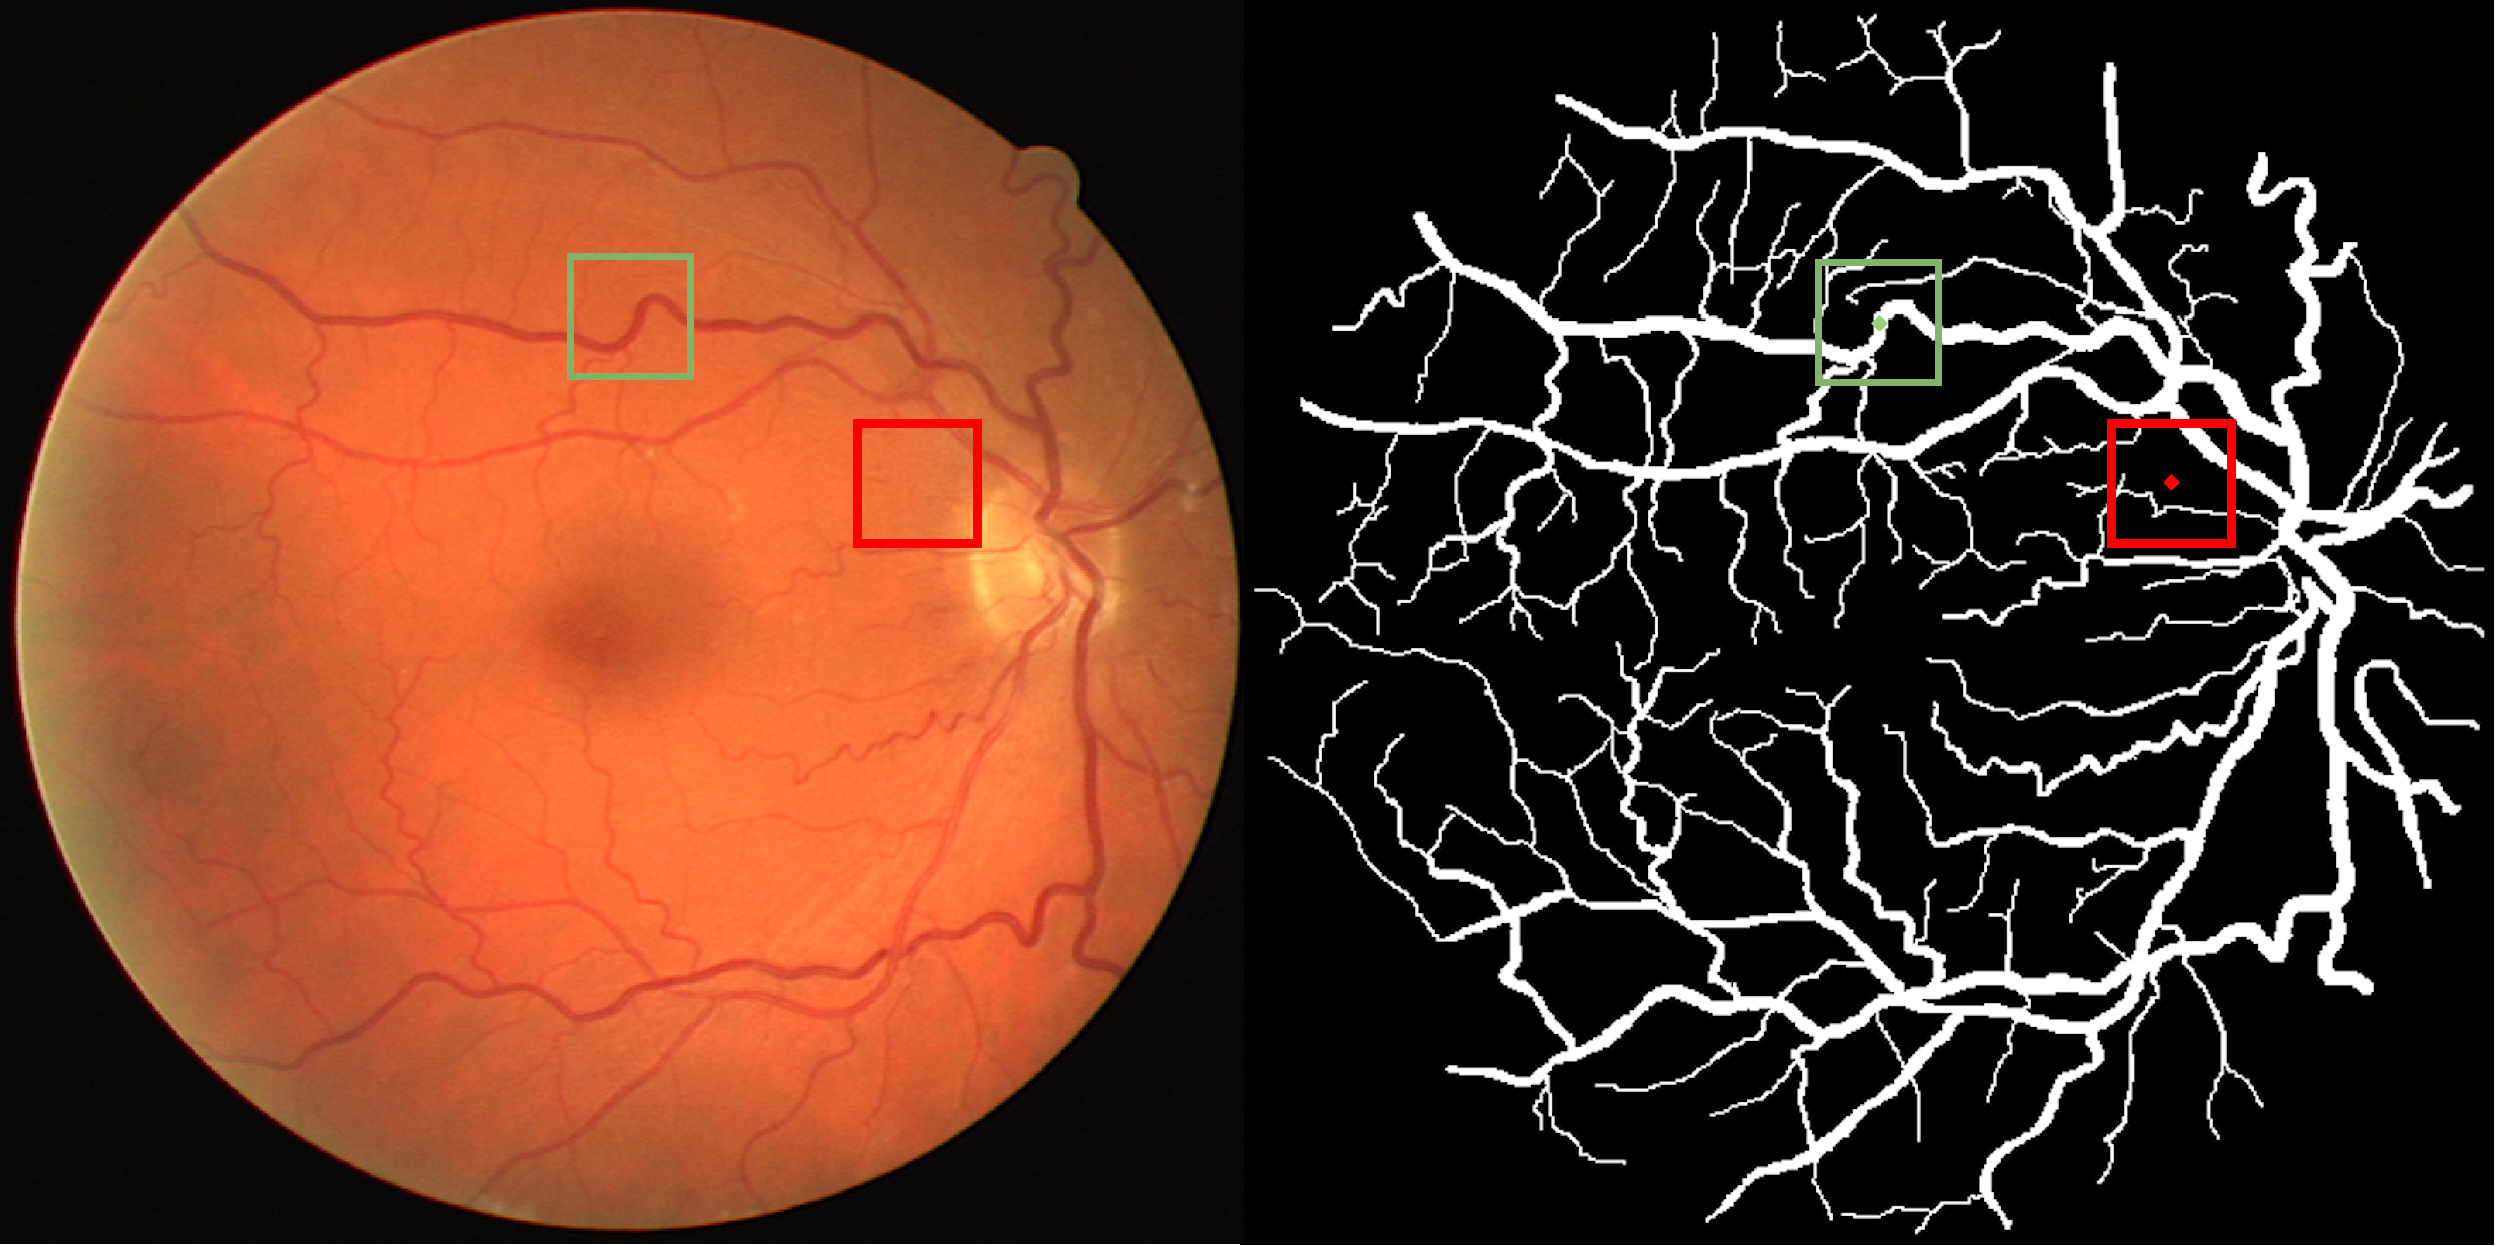
\includegraphics[width=\textwidth]{imaxes/supervision_drive.drawio.pdf}\hfill

\end{frame}

\subsection{proba de arquitecturas}
\begin{frame}
\frametitle{Proba de arquitecturas sobre Drive}
Eventualmente todas fanno parecido. Notar que as que primeiro converxen son as segundo orden con $U$ compartido, as do medio son as segundo orden sen $U$ compartido e as que máis tardan son as de primeiro orden.
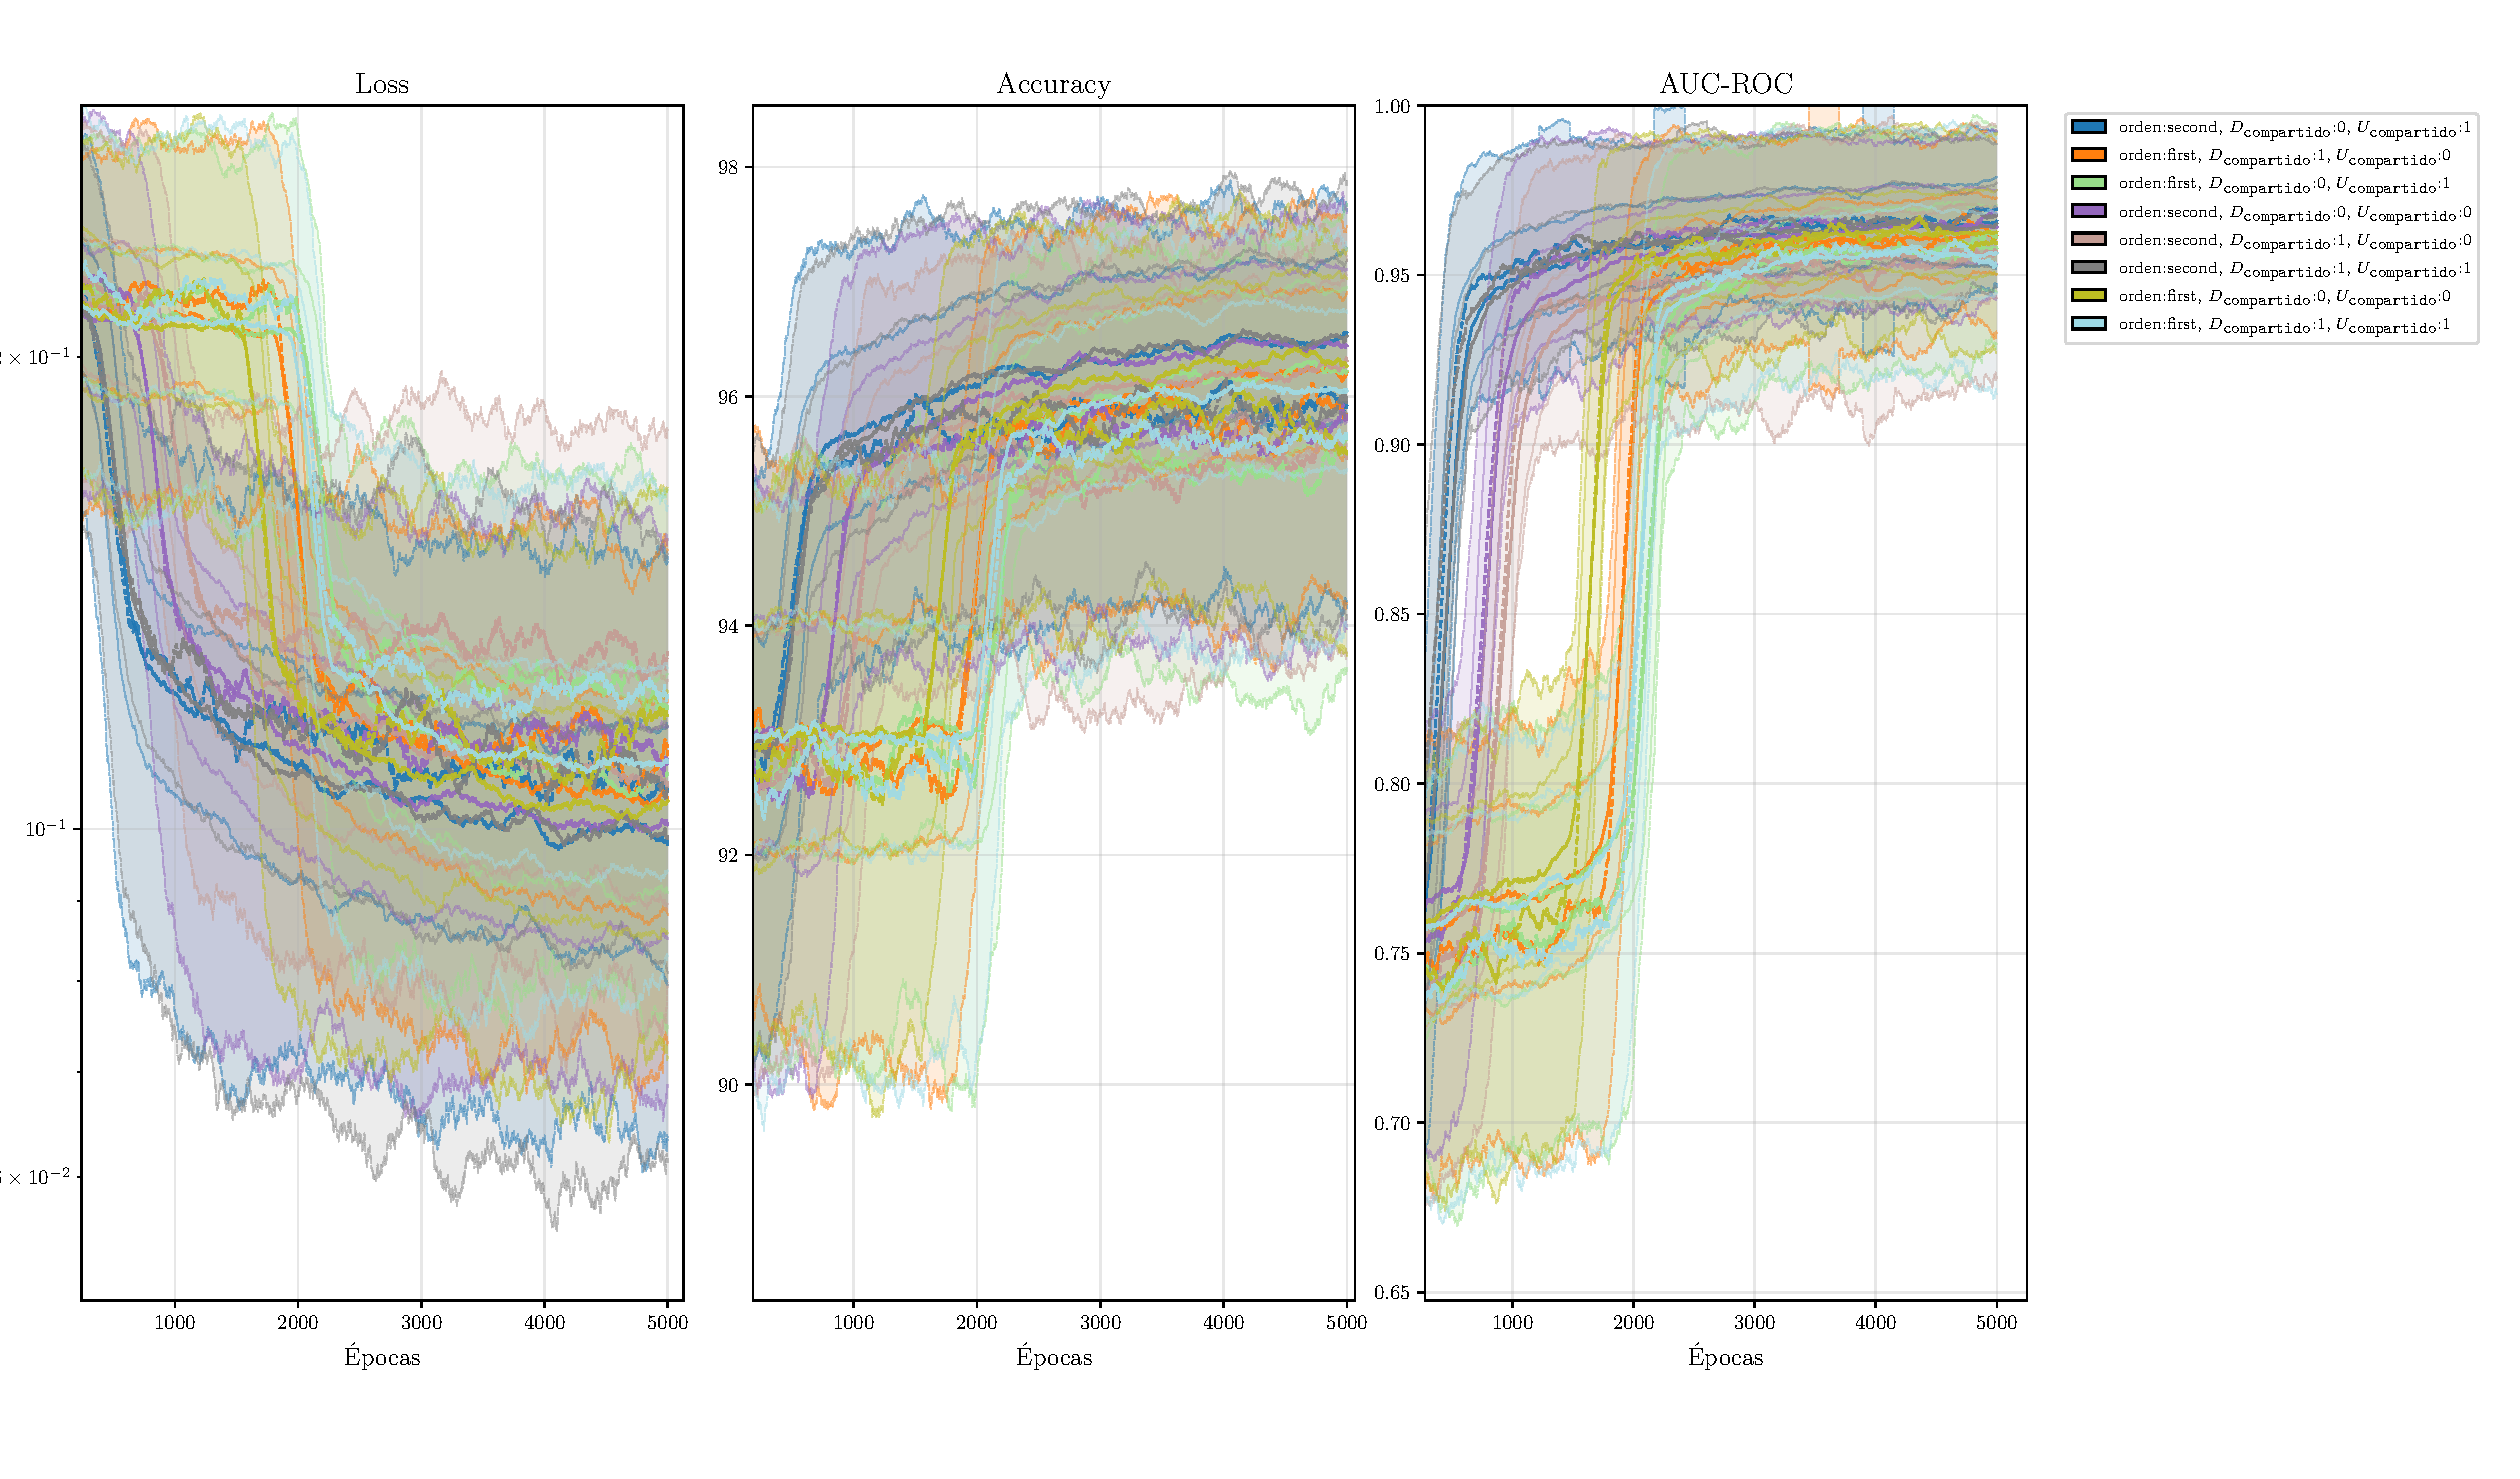
\includegraphics[width=\textwidth]{imaxes/drive_shdct4/losses.pdf}
\end{frame}

\begin{frame}
\frametitle{Proba de arquitecturas sobre Drive - mcr2 e dispersión}

Existe unha loita entre minimizar CR e maximizar a dispersión. As redes con menor CR son segundo orden (e $U$ sen compartir). As redes con maior dispersión son as de primero orden que comparten $D$

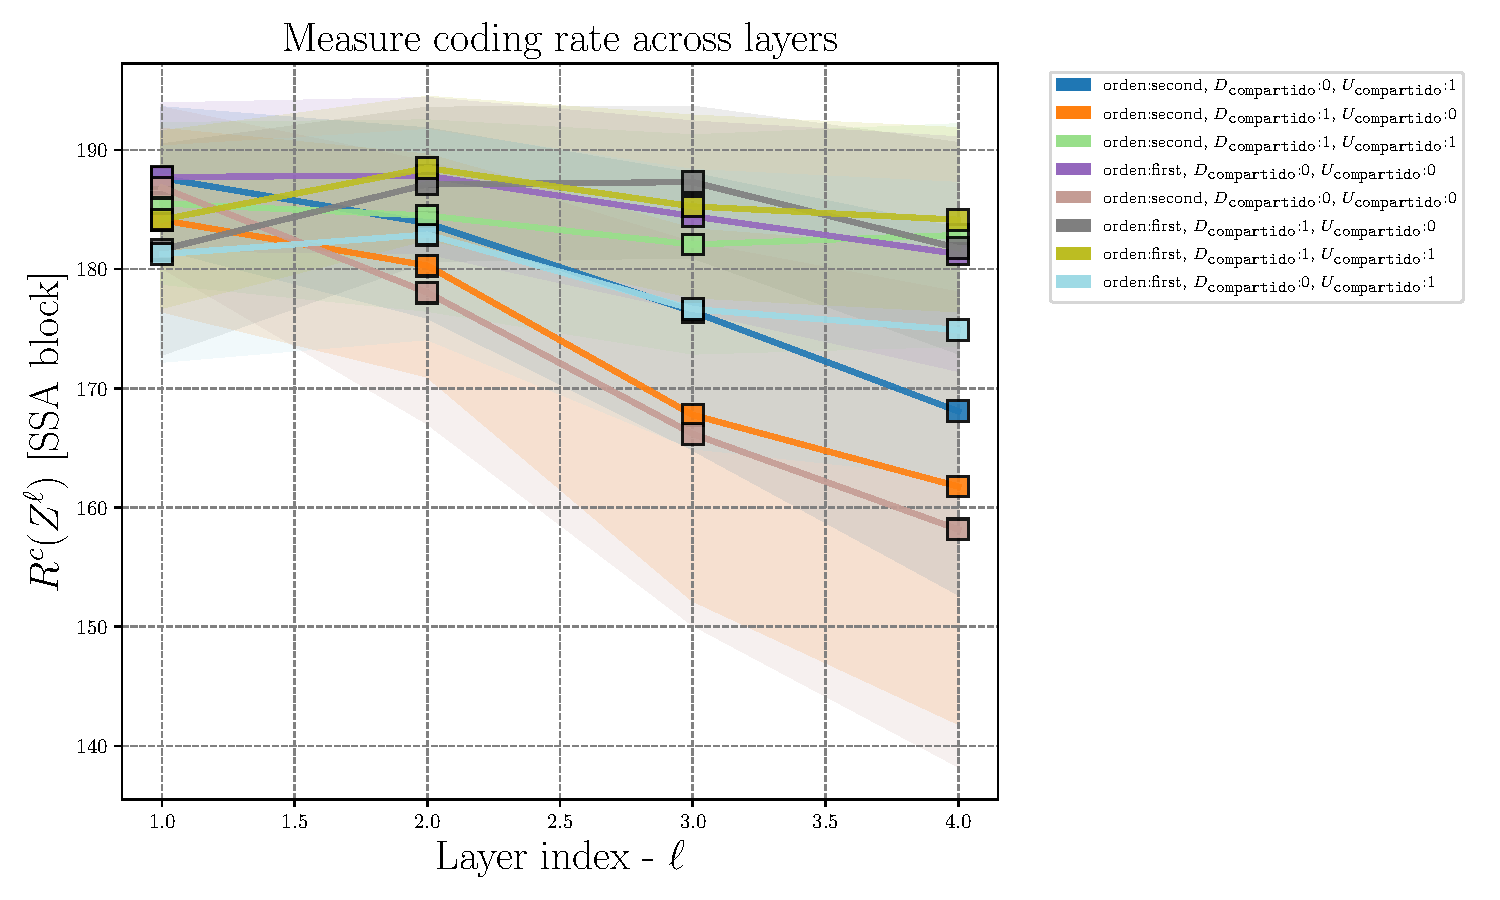
\includegraphics[width=0.48\textwidth]{imaxes/drive_shdct4/mcr2.pdf}\hfill
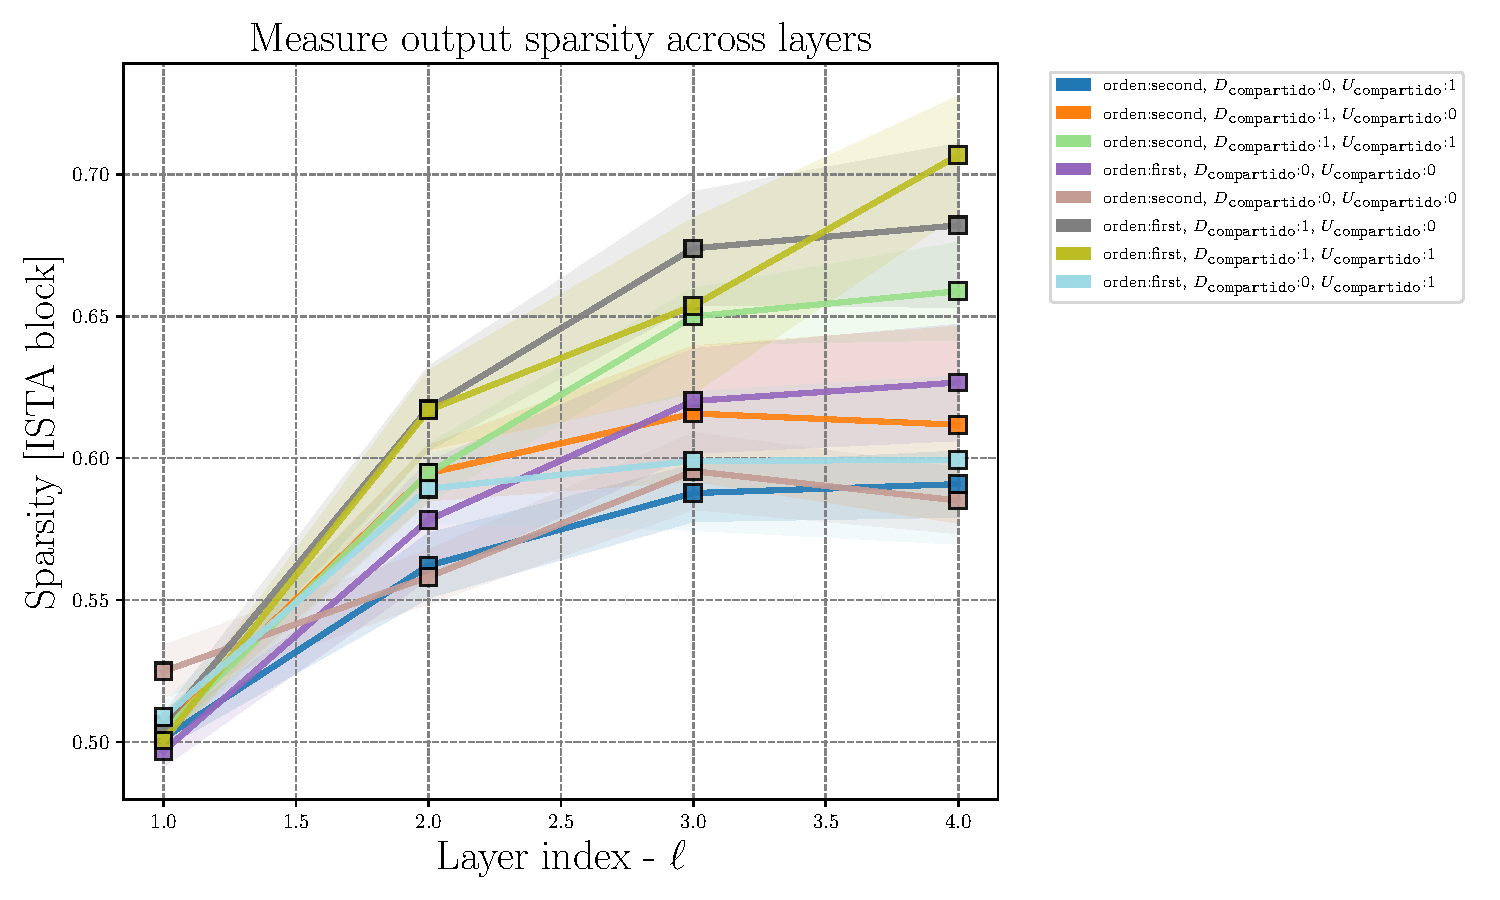
\includegraphics[width=0.48\textwidth]{imaxes/drive_shdct4/sparsity.pdf}

A \textcolor{green}{proposta combo} e en ambas métricas mellor que o \textcolor{violet}{baseline}.

\end{frame}


\begin{frame}
\frametitle{Proba de arquitecturas sobre Drive - inferencia vasos}

Non obstante tanto o baseline (izq) como a proposta combo (der) son moi malas..

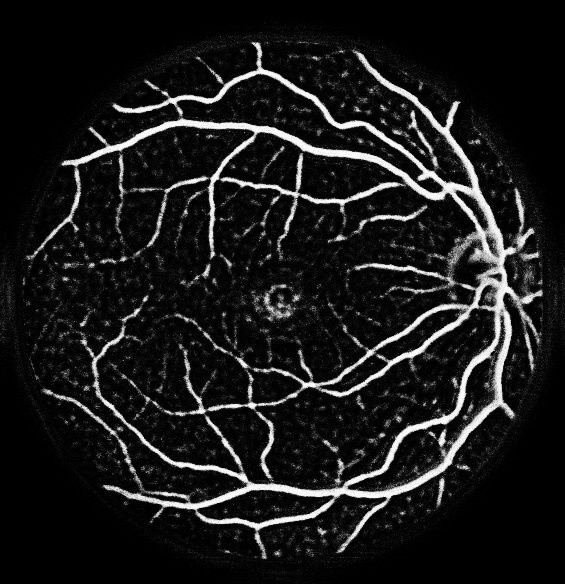
\includegraphics[width=0.45\textwidth]{imaxes/drive_shdct4/628ea0.pth_complete_inference.png}\hfill
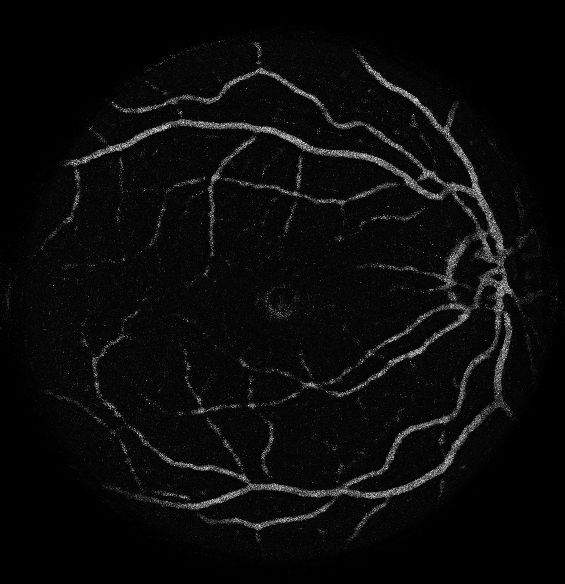
\includegraphics[width=0.45\textwidth]{imaxes/drive_shdct4/5ddaf1.pth_complete_inference.png}

Notar que aquí estanse a usar parches de 75x75 con 25 tokens de 15x15 (¿tokens moi grandes?¿poucos tokens?)
\end{frame}

\subsection{proba de tamaño token optimo}
\begin{frame}
\frametitle{Proba de tamano token optimo - curvas de aprendizaxe}

Pódese ver que canto máis pequeno tanto os tokens como o parche mellor. Eso xustifica os malos resultados anteriores.
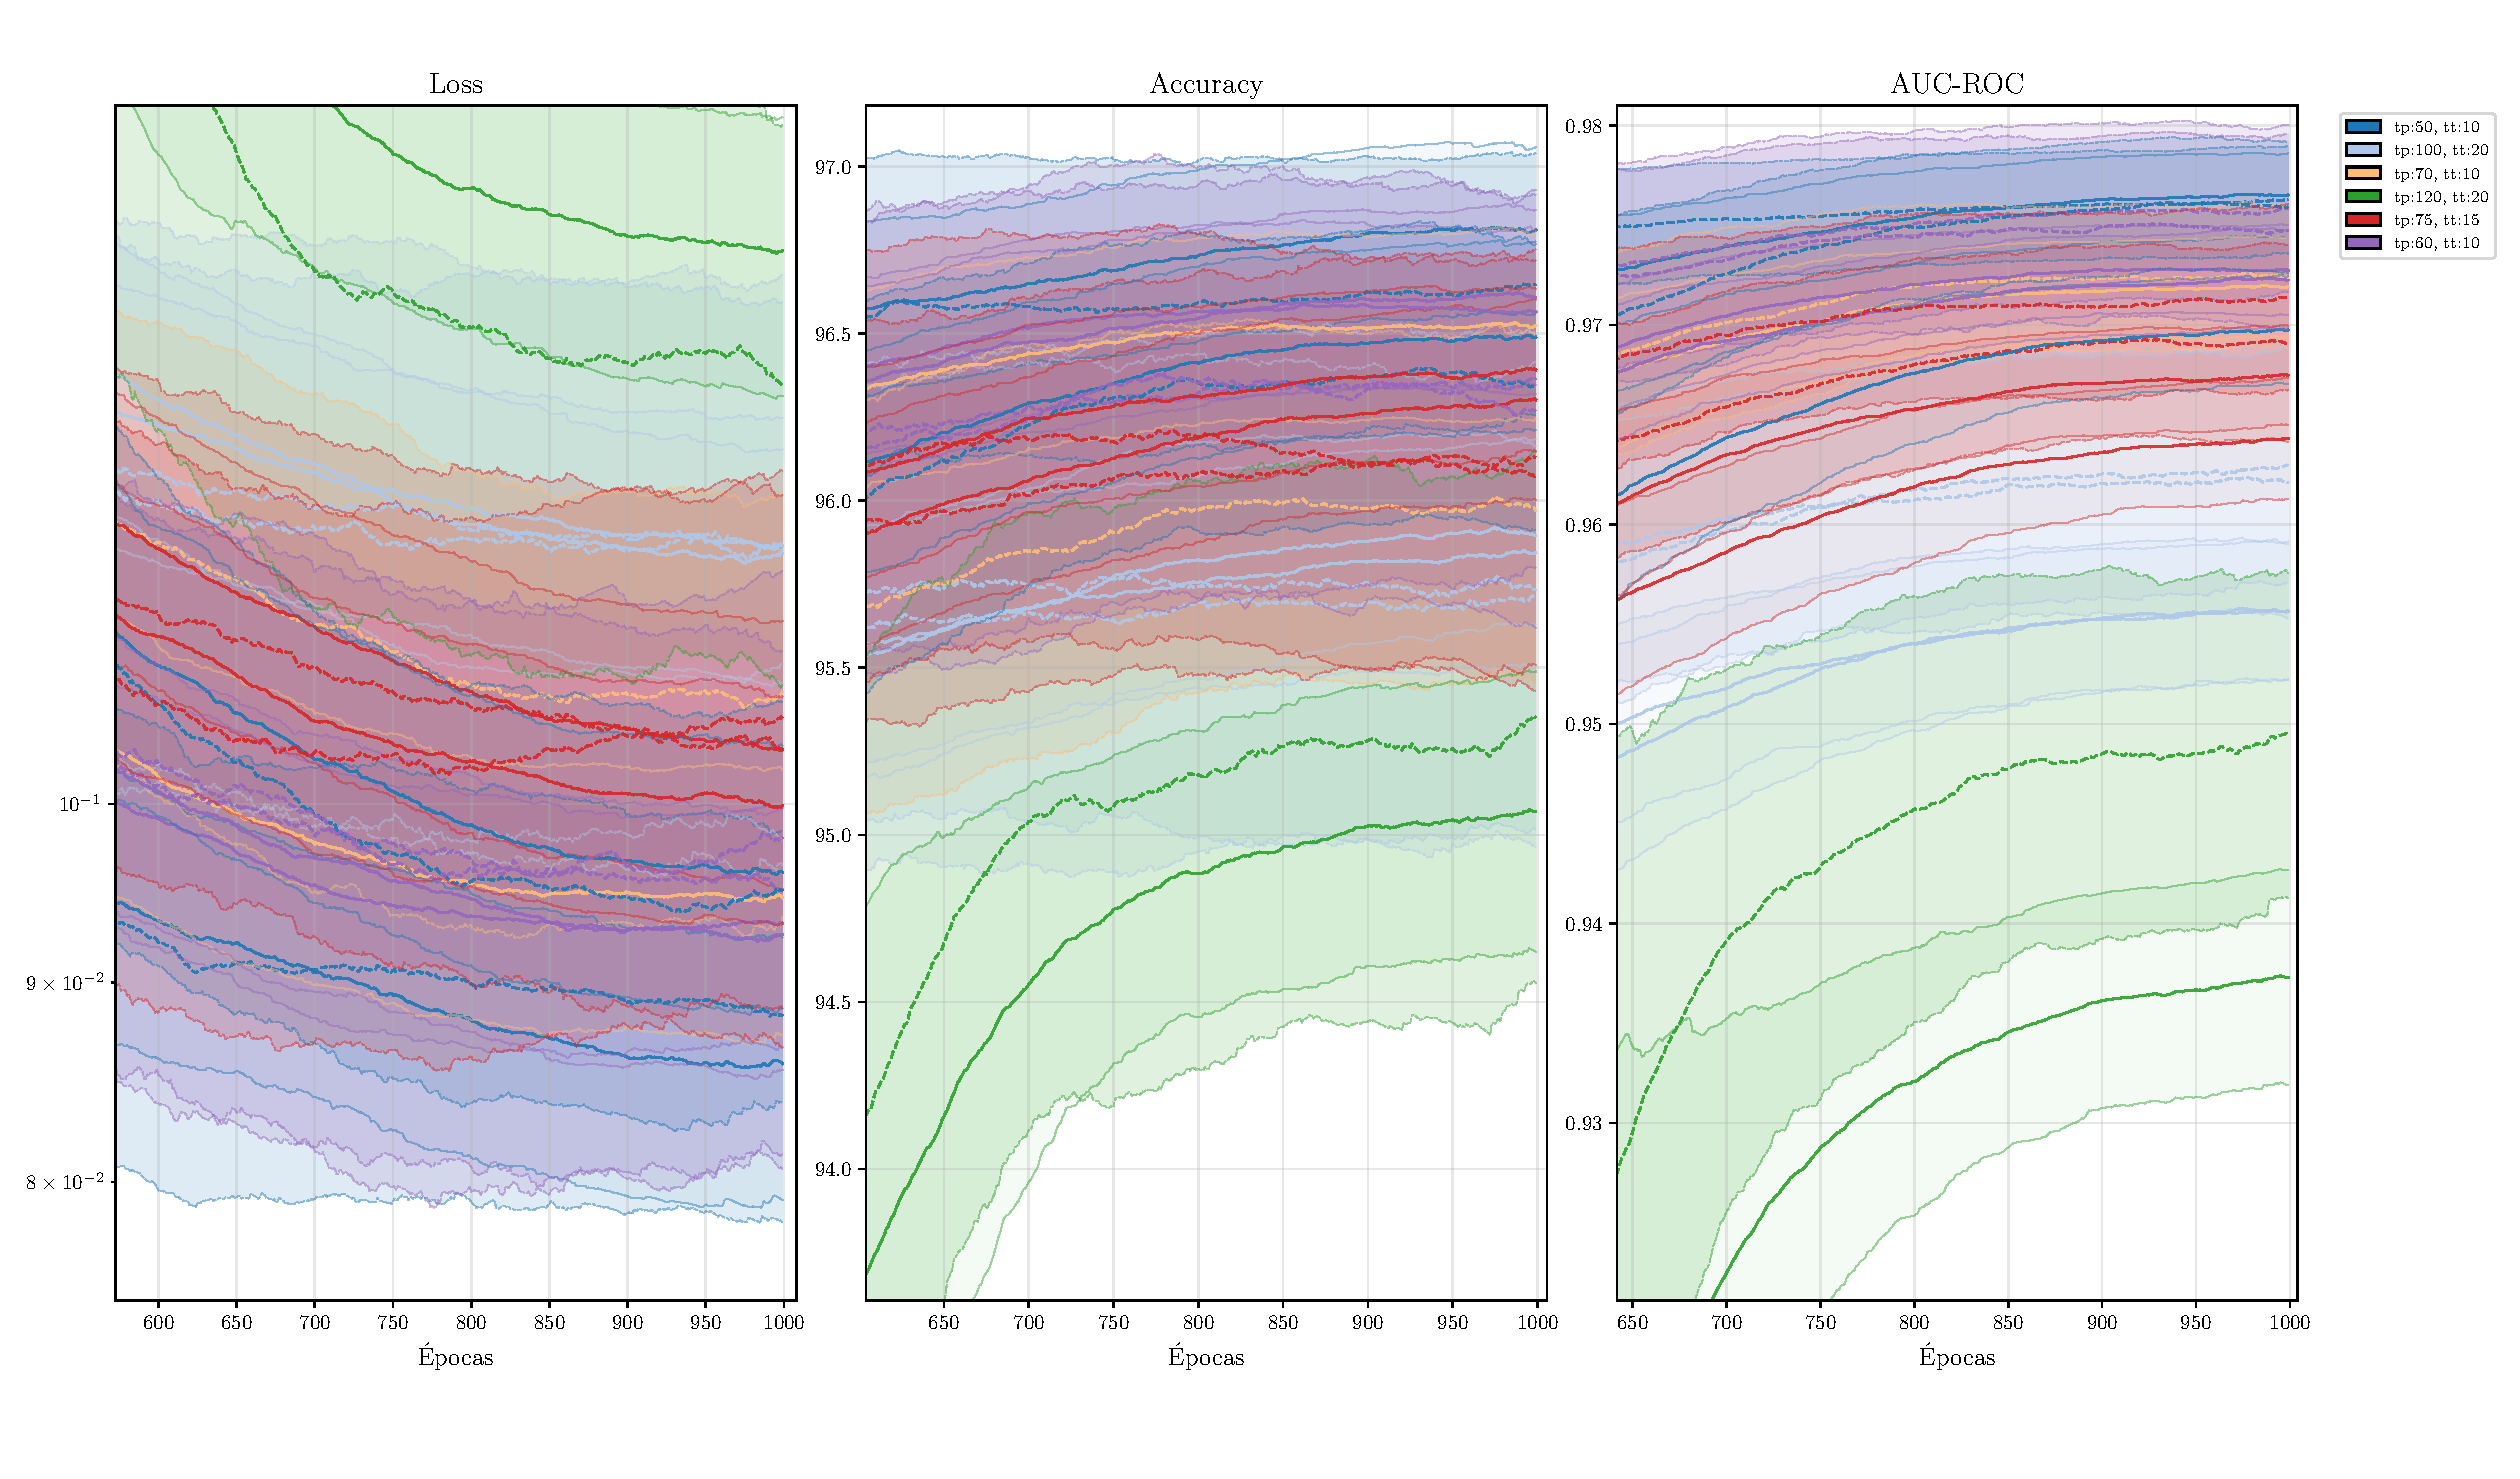
\includegraphics[width=\textwidth]{imaxes/drivetptt.pdf}

\end{frame}

\begin{frame}
\frametitle{Proba de tamano token optimo - inferencia vasos}
Tampouco son tan bos os resultados de este experimento (esta red é a que mellor segmenta do experimento; con parches de 70x70 e tokens de 10x10)
\begin{figure}
    \centering
    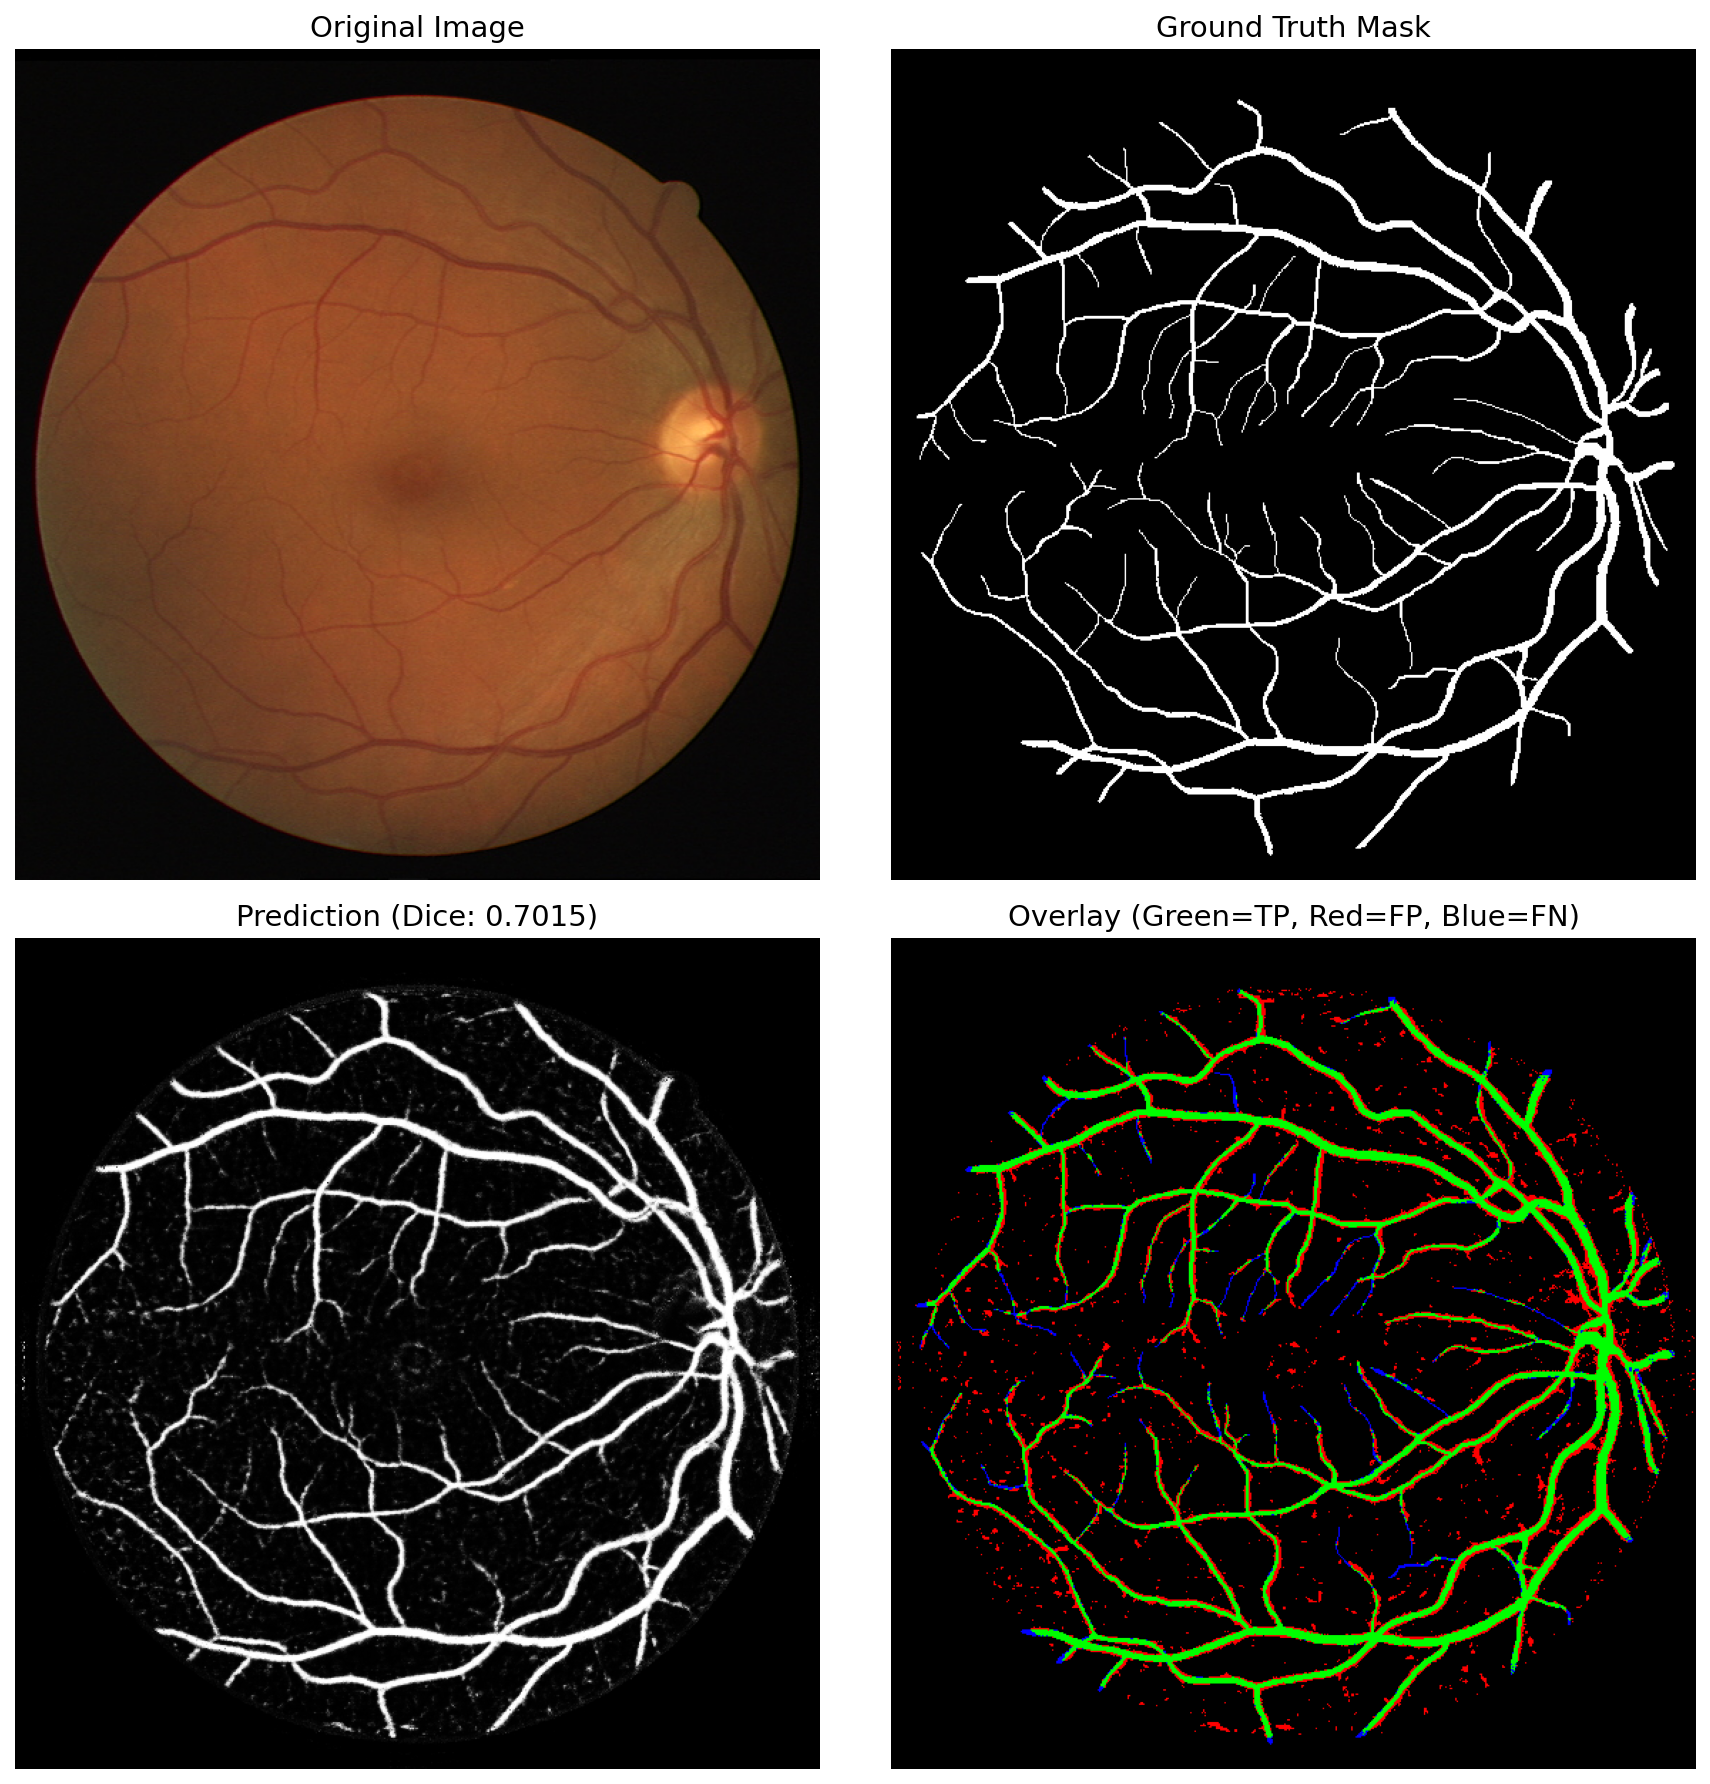
\includegraphics[
        width=\textwidth,
        height=0.7\textheight,
        keepaspectratio
    ]{imaxes/a7fec0.pth_comparison_plot.png}
\end{figure}
\end{frame}

\begin{frame}
o certo é que levaronse a cabo moitos experimentos con DRIVE, pero esencialmente as `conclusións' foron esas. Antes de rematar con DRIVE gustaríame analizar unha rede de un experimento que acabou por ter unha boa segmentación.
\end{frame}

\begin{frame}
\frametitle{Inspección de rede boa de DRIVE}

\begin{figure}
    \centering
    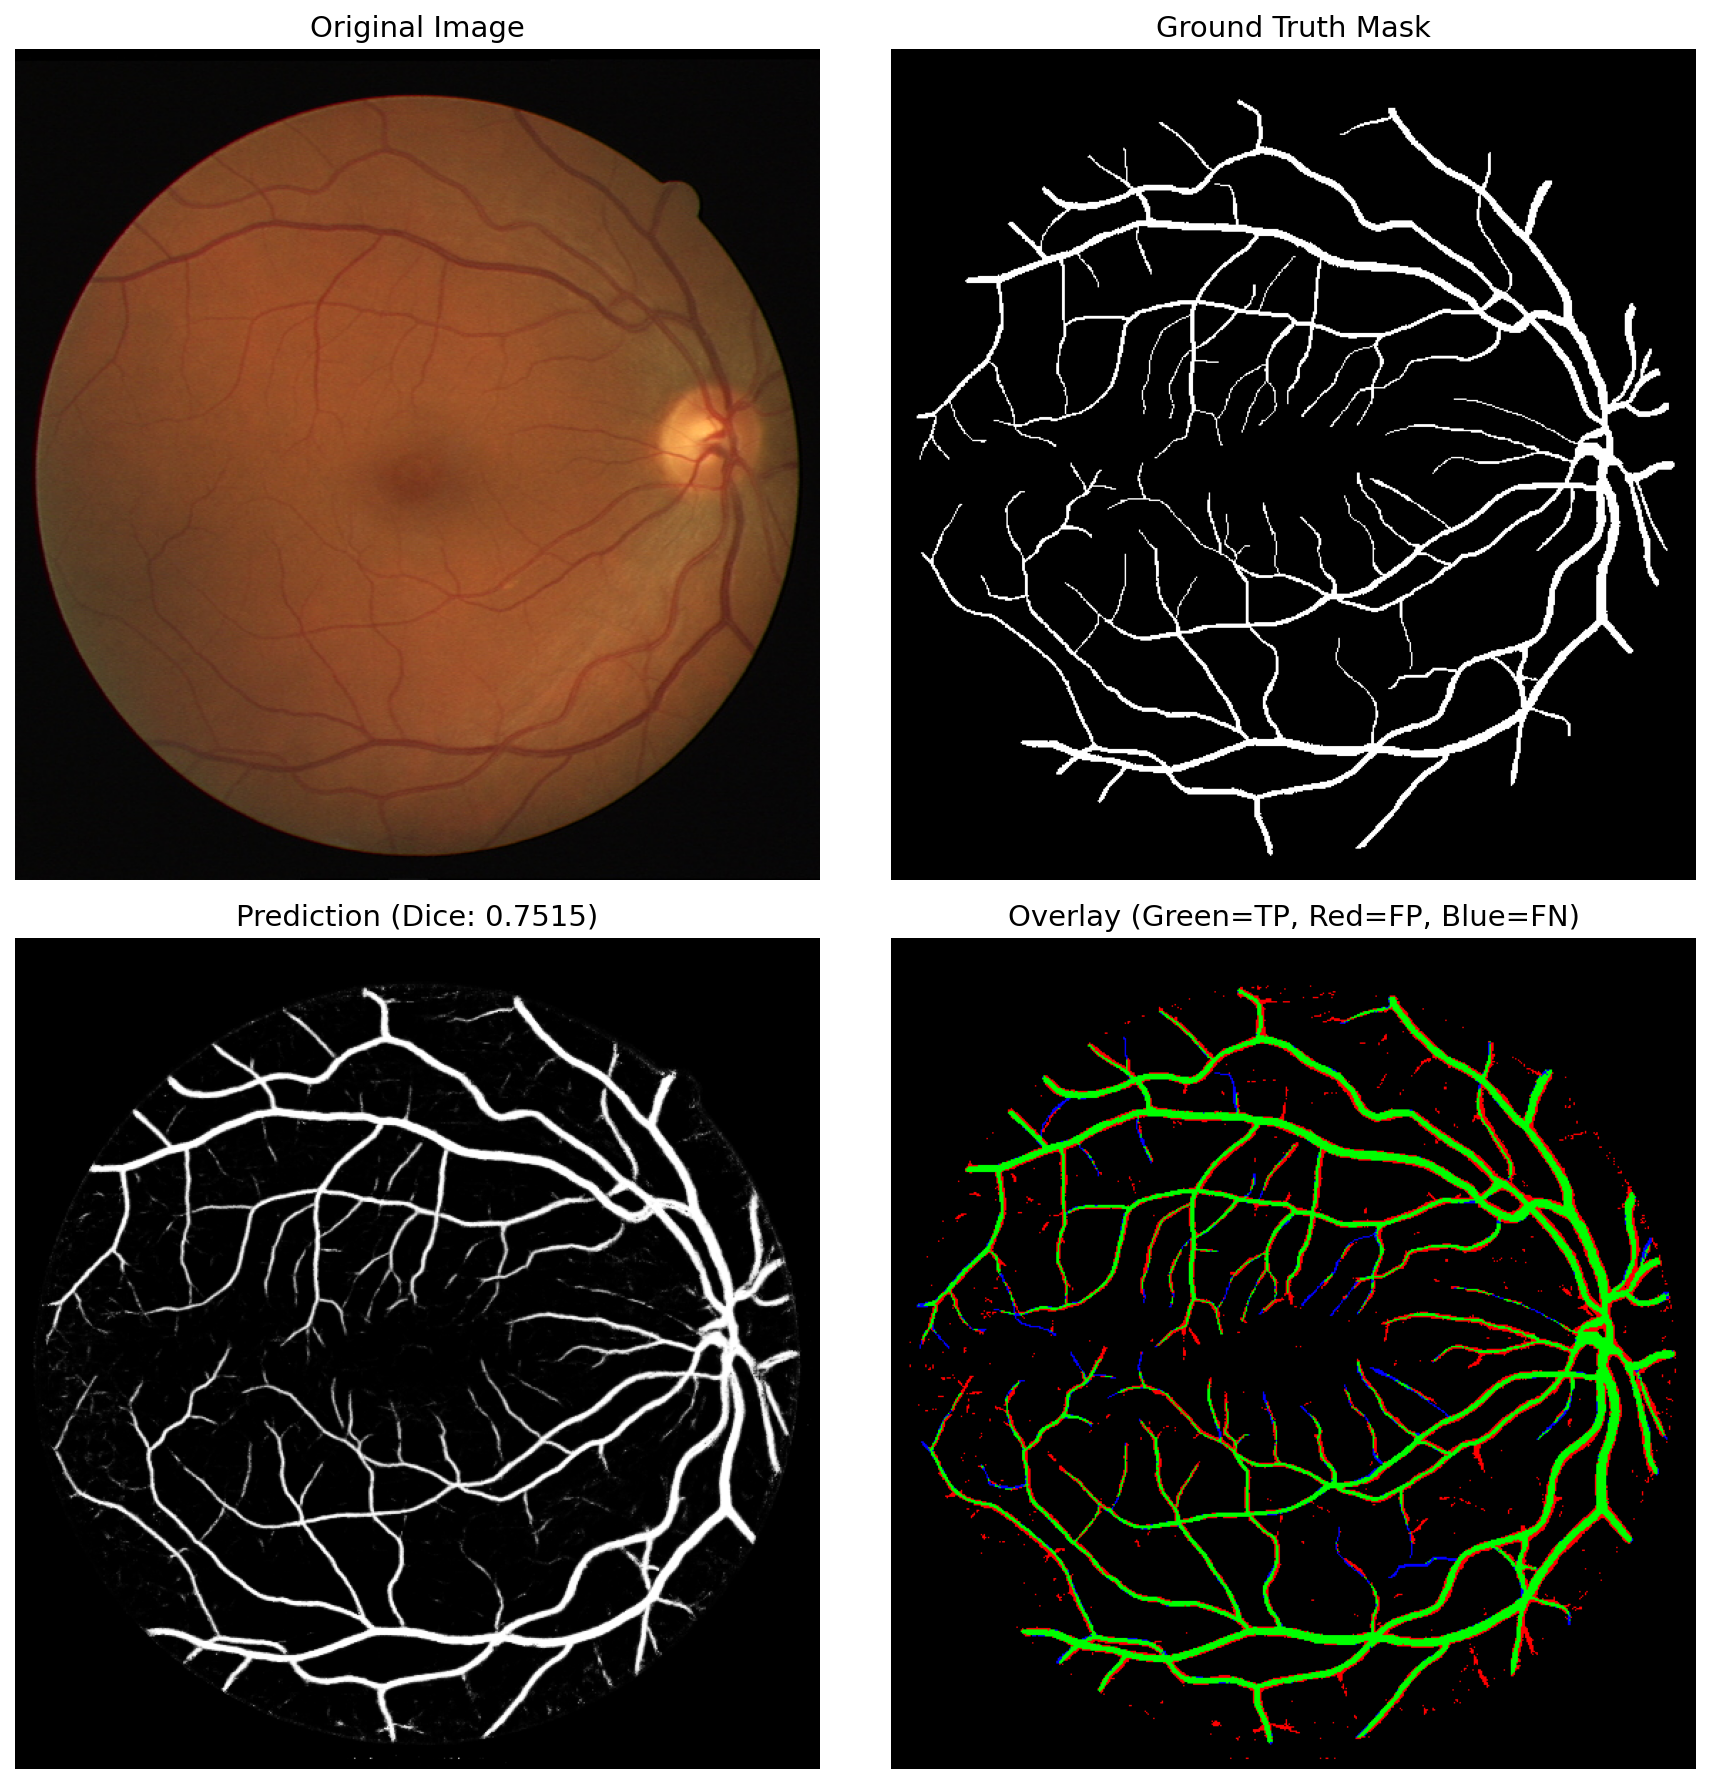
\includegraphics[
        width=\textwidth,
        height=0.9\textheight,
        keepaspectratio
    ]{imaxes/inspeccion_drive/9176ef.pth_comparison_plot.png}
\end{figure}
\end{frame}

\begin{frame}
\frametitle{Inspección de rede boa de DRIVE}

\begin{figure}
    \centering
    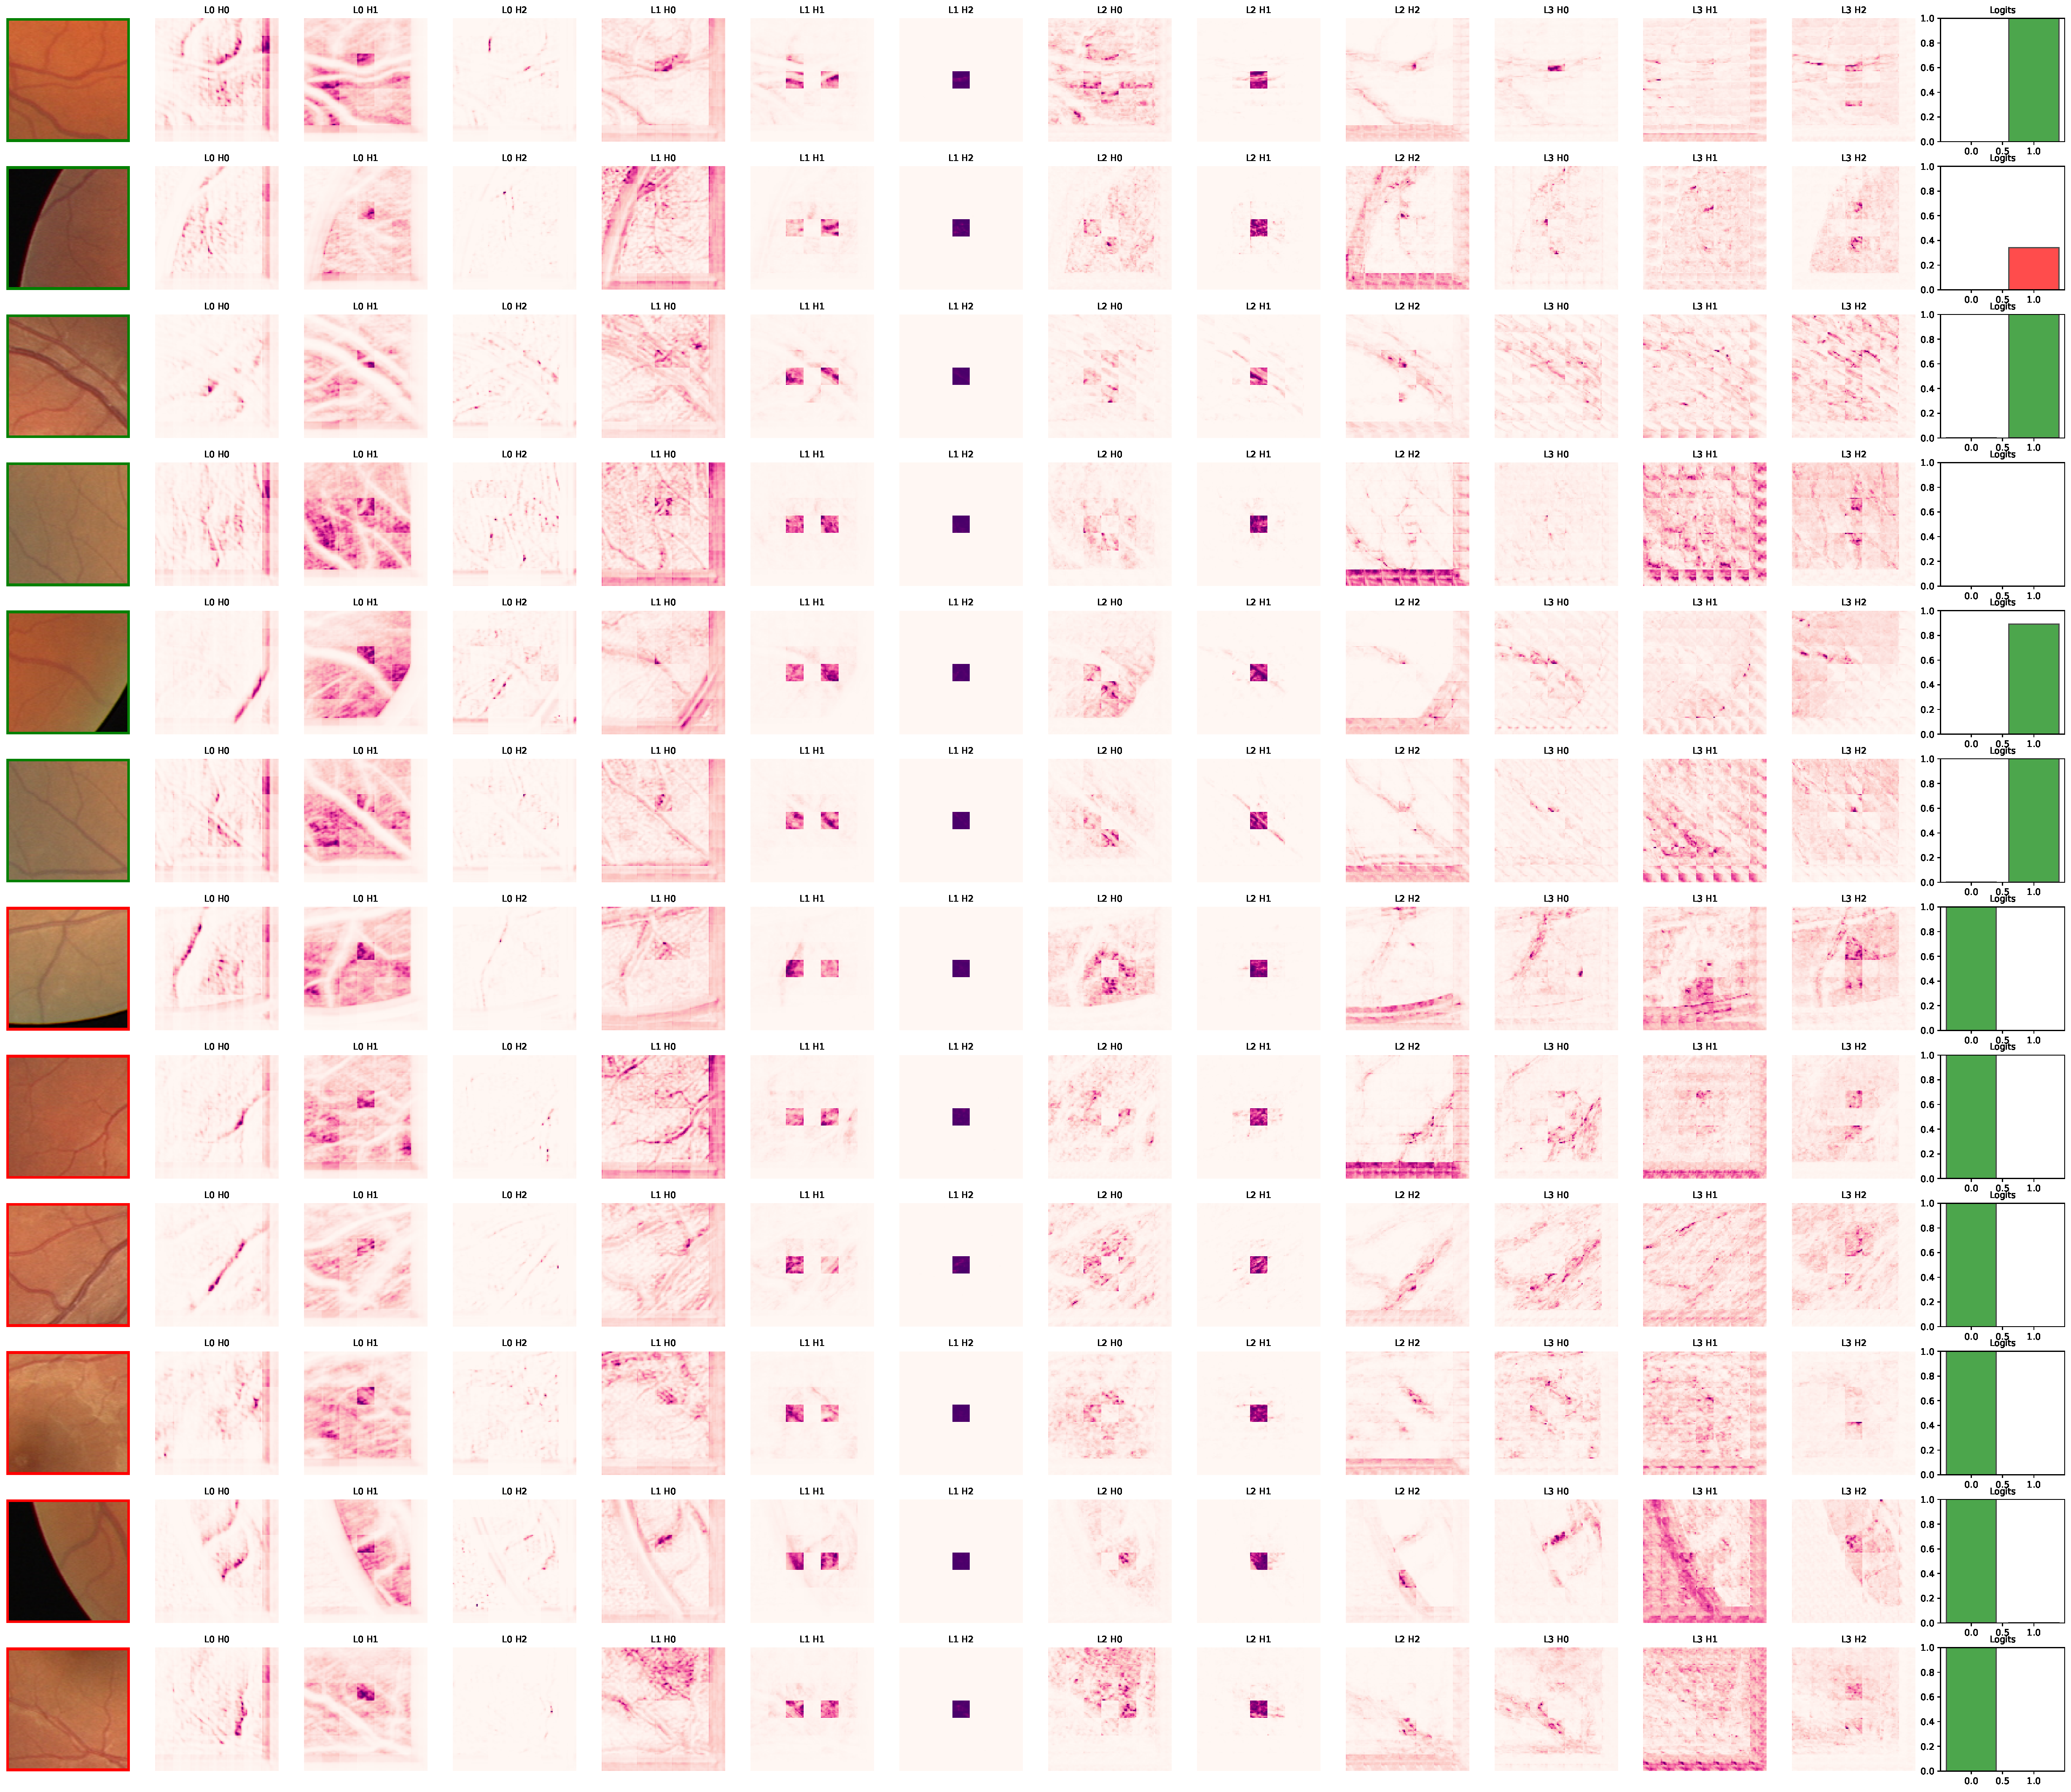
\includegraphics[
        width=\textwidth,
        height=0.9\textheight,
        keepaspectratio
    ]{imaxes/inspeccion_drive/9176ef.pth_atencion_r15.pdf}
\end{figure}
\end{frame}

\begin{frame}
\frametitle{Inspección de rede boa de DRIVE}

\begin{figure}
    \centering
    \includegraphics[
        angle=90,
        width=\textheight,
        height=\textwidth,
        keepaspectratio
    ]{imaxes/inspeccion_drive/9176ef.pth_retrieval.pdf}
\end{figure}

\end{frame}

\section{RFMiD}
\begin{frame}

A atención da mellor rede adestrada para rfmid. $\sim$2500 épocas, 97Acc en adestramento e 85Acc en validación.

\begin{figure}
    \centering
    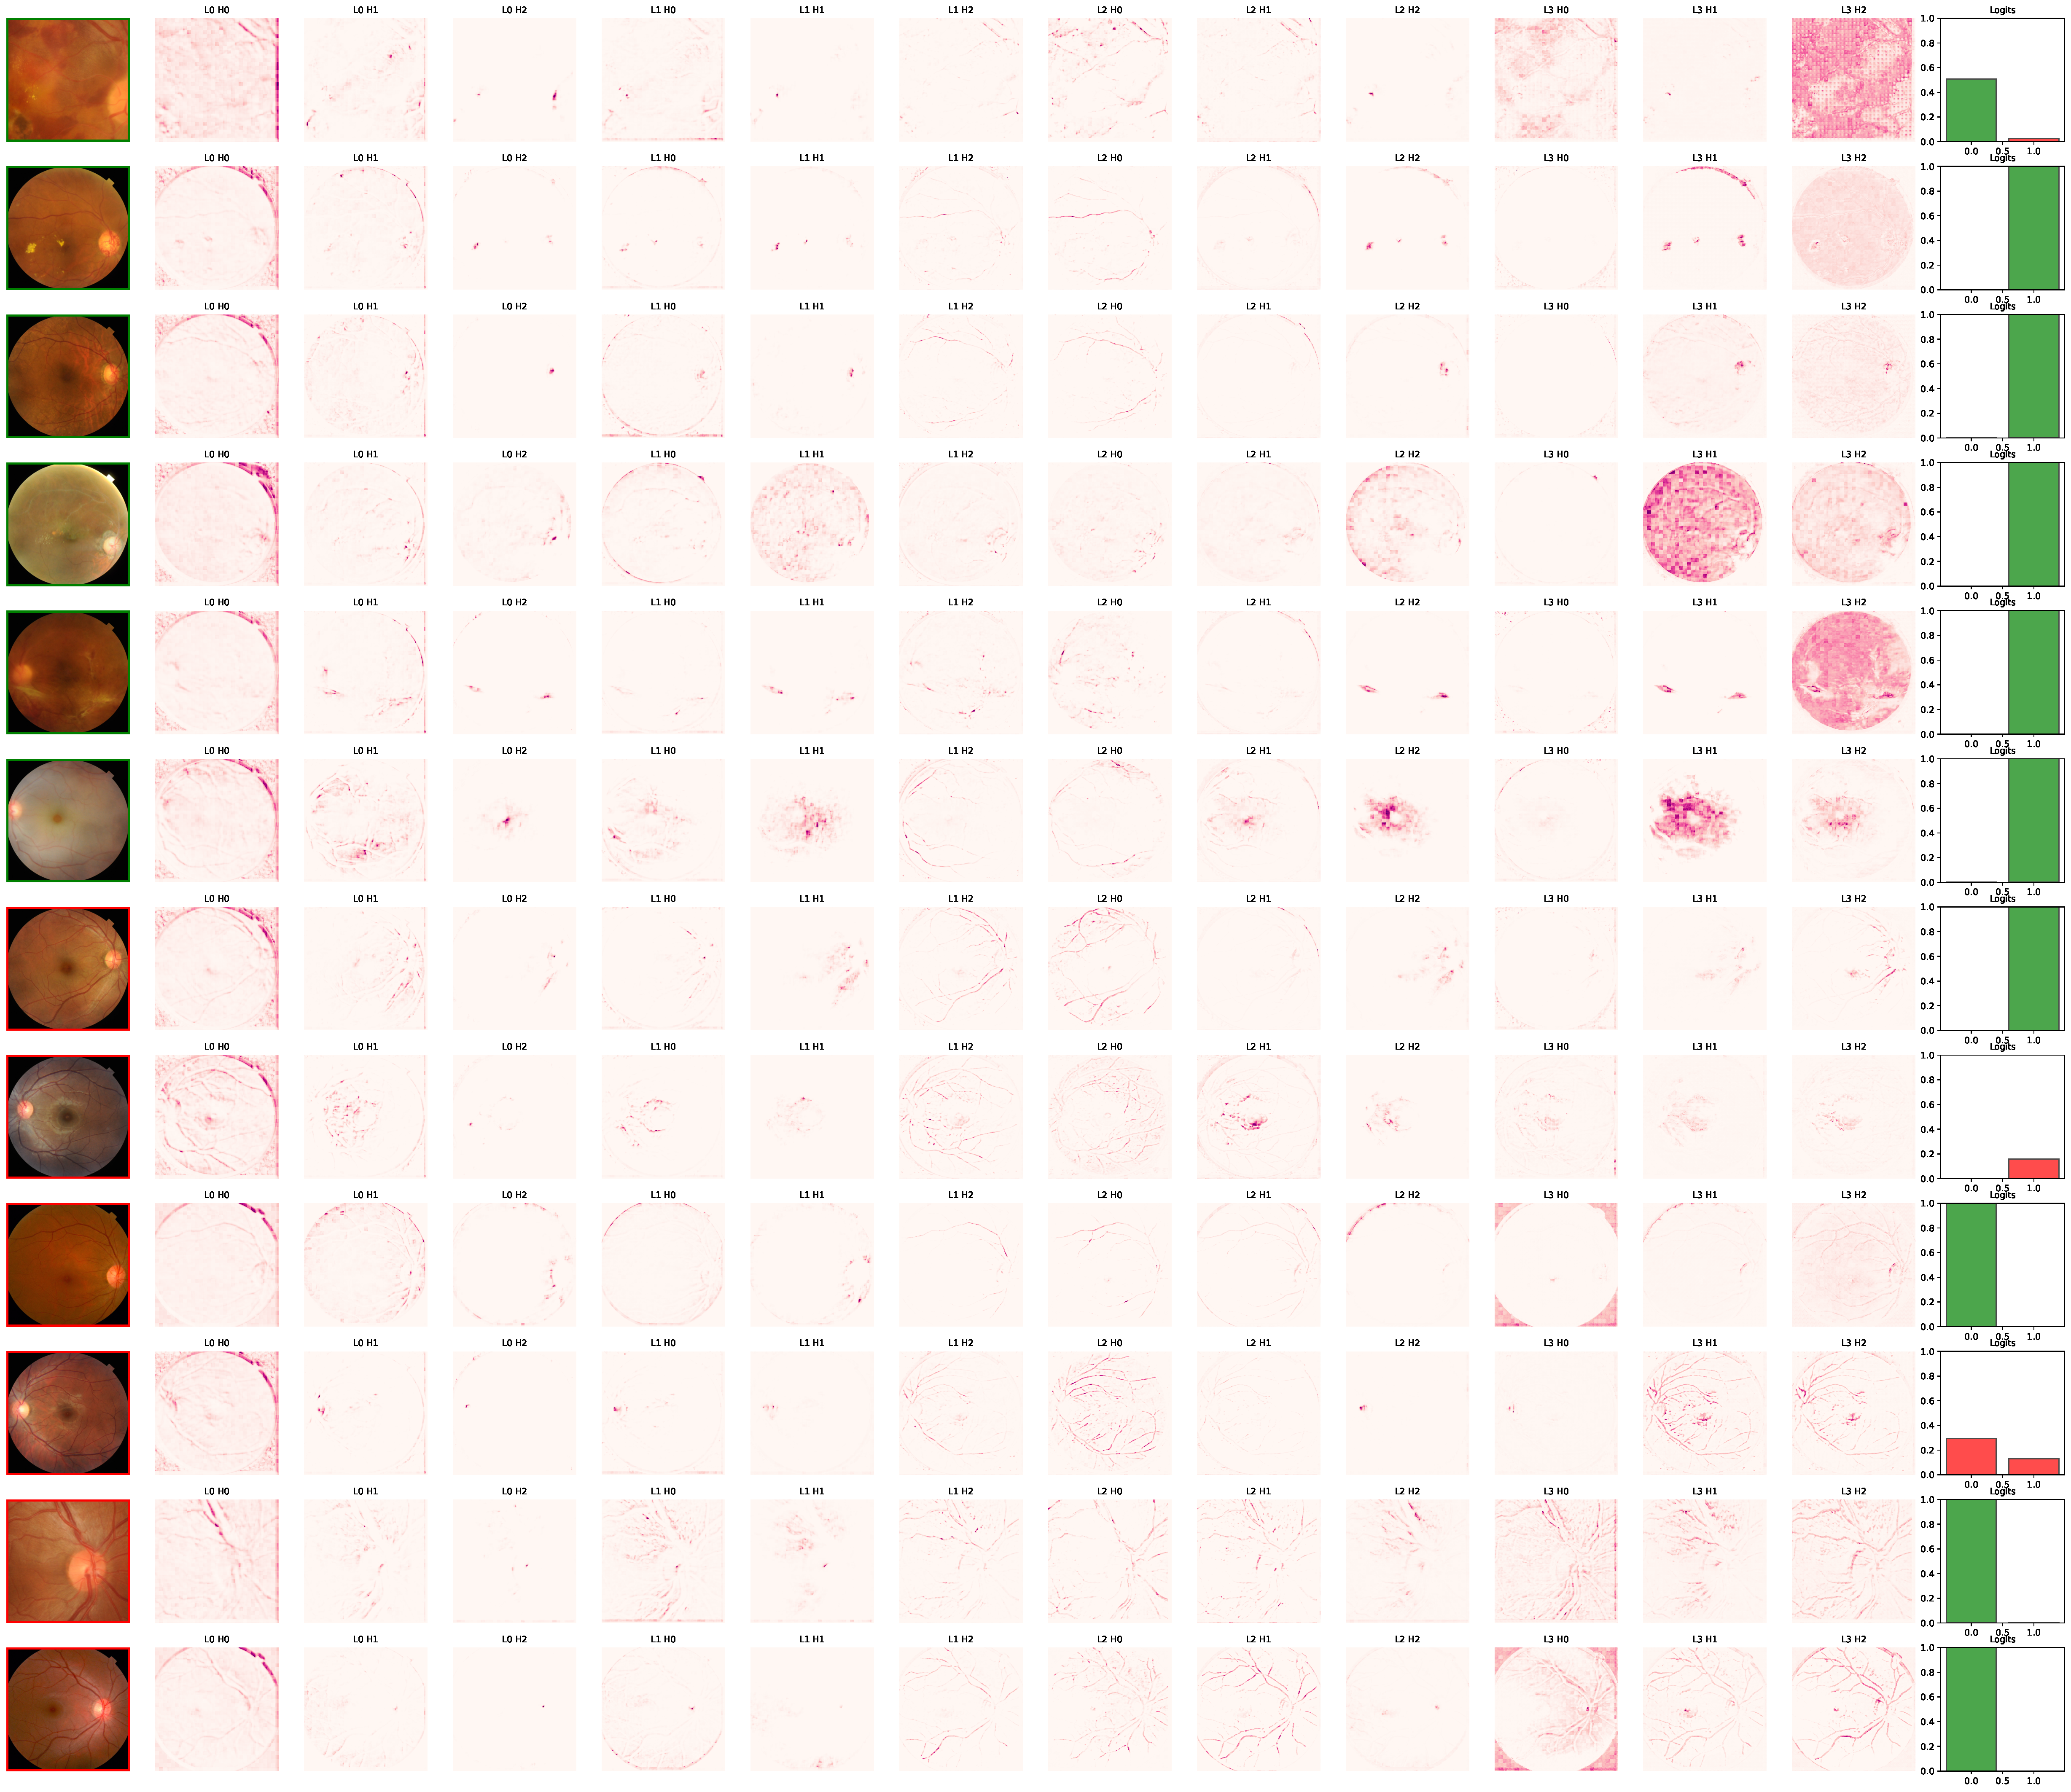
\includegraphics[
        width=\textwidth,
        height=0.9\textheight,
        keepaspectratio
    ]{imaxes/rfmid/494123.pth_atencion_r45.pdf}
\end{figure}
\end{frame}

\begin{frame}


\begin{figure}
    \centering
    \includegraphics[
        angle=90,
        width=\textwidth,
        height=0.9\textheight,
        keepaspectratio
    ]{imaxes/rfmid/494123.pth_retrieval.pdf}
\end{figure}
\end{frame}
\section{Cousas que excluín}

\begin{frame}
o linformer, o da penalización do embedding e probas marxinais para `asegurar' os hiperparametros.
\end{frame}

\end{document}
